\documentclass[11pt]{article}
\usepackage[margin=1.05in]{geometry}
\usepackage[T1]{fontenc}
\usepackage{lmodern}
\usepackage{amsmath,amssymb,amsthm,mathtools}
\usepackage{booktabs}
\usepackage{array}
\usepackage{enumitem}
\usepackage{xcolor}
\usepackage{tikz}
\usepackage[colorlinks=true,linkcolor=blue!45!black,citecolor=blue!45!black,urlcolor=blue!45!black]{hyperref}

\setlist{itemsep=2pt,topsep=4pt}


% ---------- theorem environments ----------
\newtheorem{theorem}{Theorem}[section]
\newtheorem{lemma}[theorem]{Lemma}
\newtheorem{proposition}[theorem]{Proposition}
\newtheorem{corollary}[theorem]{Corollary}
\theoremstyle{definition}
\newtheorem{definition}[theorem]{Definition}
\theoremstyle{remark}
\newtheorem{remark}[theorem]{Remark}
\theoremstyle{plain}
\newcommand{\namedthmname}{}
\newtheorem*{namedthminner}{\namedthmname}
\newenvironment{named}[1]{\renewcommand{\namedthmname}{#1}\begin{namedthminner}}{\end{namedthminner}}

% ---------- notation ----------
\newcommand{\PM}{\mathrm{PM}}
\newcommand{\TV}{\mathrm{TV}}
\newcommand{\BC}{\mathrm{BC}}
\newcommand{\E}{\mathbb{E}}
\newcommand{\R}{\mathbb{R}}
\newcommand{\C}{\mathbb{C}}
\newcommand{\Z}{\mathbb{Z}}
\newcommand{\eps}{\varepsilon}
\newcommand{\prof}{\operatorname{prof}}
\newcommand{\tr}{\operatorname{tr}}
\newcommand{\sgn}{\operatorname{sgn}}
\newcommand{\asinh}{\operatorname{asinh}}
\newcommand{\rank}{\operatorname{rank}}
\newcommand{\vars}{\operatorname{vars}}
\newcommand{\supp}{\operatorname{supp}}
\newcommand{\OPT}{\mathrm{OPT}}
\newcommand{\norm}[1]{\lVert #1\rVert}
\newcommand{\abs}[1]{\lvert #1\rvert}
\newcommand{\cA}{\mathcal{A}}
\newcommand{\cB}{\mathcal{B}}
\newcommand{\cU}{\mathcal{U}}
\newcommand{\cT}{\mathcal{T}}
\newcommand{\one}{\mathbf{1}}
\emergencystretch=3em
\newcommand{\ket}[1]{\lvert #1\rangle}
\newcommand{\bra}[1]{\langle #1\rvert}

\title{Uniform square-grid dimers versus monotone and nonnegative circuits}
\author{Chris Blaschke\\Ax0s}
\date{November 3, 2026. Preprint, not peer reviewed.\\ \small Source, numerical checks and release history: \url{https://github.com/chrisblaschke/square-grid-dimers}}

\begin{document}
\maketitle

\begin{abstract}
Valiant (1980) proved that monotone arithmetic circuits for the perfect-matching polynomial of a triangular grid need exponential size. He noted that one step of his argument fails for rectangular grids, so their monotone complexity was left open. We settle the square case. Let $U_L$ be the uniform distribution on the domino tilings of the free $L\times L$ square ($L$ even), viewed as a distribution on the $n=2L(L-1)$ edge indicators. For every split of the edges into two parts of size at least $n/3$, and every vertex set $S$, the probability that the matching edges in the first part cover exactly $S$ is at most $\exp(-L/1129)$ once $L\ge 1000$. The same bound holds for the probability that no matching edge leaves a vertex set of size between $L^2/3$ and $2L^2/3$. The proof uses a tilted Kasteleyn determinant, Carleman's determinant inequality, and an elementary bound $\abs{K^{-1}(w,b)}\le 4A/\norm{w-b}_\infty$ for the free square with an explicit constant $A\approx1.37$.

Three consequences follow. (i) Monotone arithmetic circuits and $(\min,+)$ circuits for the square-grid matching polynomial need size $\exp(\Omega(L))$, which matches an $\exp(O(L))$ upper bound. (ii) Every nonnegative, smooth, decomposable probabilistic circuit with leaves of arity at most $2n/3$ and within total variation $\eps<1$ of $U_L$ has size at least $(1-\eps)^2e^{cL}$. A column-transfer circuit of size $O(L^2(1+\sqrt2)^L)$ is exact, so the optimal size in this class is $\exp(\Theta(\sqrt n))$ for every fixed error below one. (iii) The Rokhsar--Kivelson dimer state on the square has R\'enyi-$\infty$ entropy at least $cL$ across every balanced link bipartition. $U_L$ also has polynomial-size determinant-based generating circuits, and exact inference for it is easy. We specify which signed circuit classes this does and does not cover. A triangular-grid analogue of (ii) already follows from Valiant's argument, and we state it first. What is new here is the square-grid package.
\end{abstract}

\tableofcontents

\section{Introduction}\label{sec:intro}

For a graph $G=(V,E)$ with one variable $z_e$ per edge, the perfect-matching polynomial is
\[
  P_G(z)=\sum_{M\in\PM(G)}\ \prod_{e\in M} z_e .
\]
Valiant~\cite{Valiant80,Valiant79} studied a family of triangular grids $G_r$ with $\Theta(r^2)$ vertices. He proved that every monotone arithmetic circuit for $P_{G_r}$, meaning one with no subtraction, has size at least $c^r$ for a constant $c>1$ \cite[Thm.~1]{Valiant80}. With subtraction, Kasteleyn's Pfaffian method computes $P_{G_r}$ with polynomially many operations \cite[Thm.~2]{Valiant80}. The lower bound relies on a local property of the triangular lattice, his Lemma~8. On the last page he writes:
\begin{quote}
``In conclusion we note that our Lemma 8 is false for regular rectangular grids. The monotone complexity of these closely related polynomials is therefore unresolved.'' \cite[p.~313]{Valiant80}
\end{quote}

This paper treats the free $L\times L$ square grid with $L$ even. We write $P_L$ for its perfect-matching polynomial and $U_L$ for the uniform distribution on its perfect matchings (domino tilings), viewed as a distribution on $\{0,1\}^n$ with $n=2L(L-1)$ edge indicators. Throughout, $0\le\eps\le1$ denotes a total-variation error. We prove the following.
\begin{itemize}
\item Every monotone arithmetic circuit for $P_L$, and every $(\min,+)$ circuit for the minimum-weight perfect matching on the grid, has size at least $\exp(c(L)L)$. Here $c(L)\ge 1/1129$ for $L\ge1000$. A transfer-matrix circuit of size $O(L^2(1+\sqrt2)^L)$ shows that this is tight up to the constant in the exponent (Theorems~D and~C).
\item Every nonnegative, smooth, decomposable probabilistic circuit (PC) with leaves of arity at most $2n/3$ whose distribution is within total variation $\eps<1$ of $U_L$ has size at least $(1-\eps)^2\exp(c(L)L)$. Determinism is not assumed (Theorem~B). So the optimal size of such circuits is $\exp(\Theta(L))=\exp(\Theta(\sqrt n))$, both for exact representation and for every fixed error below one.
\end{itemize}
Both lower bounds rest on one probability estimate, Theorem~A and its vertex-cut variant Theorem~A$'$. For every split $E=A\sqcup B$ of the edges with $\abs A,\abs B\ge n/3$ and every vertex set $S$,
\[
  U_L\bigl(\text{the edges of } M \text{ in } A \text{ cover exactly } S\bigr)\ \le\ e^{-c(L)L}.
\]
For the Rokhsar--Kivelson state on the square this says that the R\'enyi-$\infty$ entropy is at least $c(L)L$ across every balanced bipartition of the links (Corollary~\ref{cor:entanglement}).

We have not found a later resolution of the square case in the literature. Our search (Section~\ref{sec:related}) was targeted, not exhaustive.

\subsection{What already follows from Valiant's argument}\label{sec:intro-triangular}

A robust separation of the same kind already follows from Valiant's proof, so we state it first. The intermediate counting statement in his proof of Theorem~1 \cite[pp.~311--312]{Valiant80} is stronger than the theorem. For every vertex partition of $G_r$ into two parts of comparable size, the fraction of perfect matchings with no edge across the partition is $\exp(-\Omega(r))$. Section~\ref{sec:vertex-route} shows that such a counting statement, combined with standard degree homogenization and an overlap bound, gives a constant-TV lower bound for nonnegative decomposable PCs with univariate leaves.

\begin{proposition}[Valiant's argument, robust form]\label{prop:triangular}
Let $G_r$ be Valiant's triangular grid, with $r(r+1)/2$ vertices, for those $r$ where it has perfect matchings. Let $T_r$ be the uniform distribution on its perfect matchings, as a distribution on edge indicators. There are constants $c_0>0$ and $r_0$ such that for $r\ge r_0$:
\begin{enumerate}[label=(\alph*)]
\item every nonnegative smooth decomposable PC with univariate leaves whose distribution $Q$ satisfies $\TV(T_r,Q)\le\eps$ has size at least $(1-\eps)^2e^{c_0r}/\mathrm{poly}(r)$;
\item the generating polynomial $\sum_x T_r(x)z^x$ has an arithmetic circuit of size $\mathrm{poly}(r)$ that uses subtraction, that is, a polynomial-size probabilistic generating circuit in the sense of~\cite{ZhangJubaVdB21}.
\end{enumerate}
For every fixed error below one, part (a) gives size $\exp(\Omega(r))$.
\end{proposition}

Part (b) is Valiant's Theorem~2 after normalization: Kasteleyn's Pfaffian gives every matching the same sign. Part (a) combines Valiant's Lemmas~6--8 and Corollary~9, as used in his proof of Theorem~1, with two standard steps. The proof is in Section~\ref{sec:vertex-route}. We have not found (a) stated in this form. It is still best read as a corollary of 1980 techniques. In particular, the existence of an exponential constant-TV gap between nonnegative decomposable PCs and determinant-based circuits on a natural planar lattice is not new. Generic separations of this type with $\exp(\Omega(n))$ size also follow from older code constructions (Section~\ref{sec:codes}). The contribution of this paper is the square-grid package: Theorems~A, A$'$, B, C and D, and the analytic proof behind them.

\subsection{What fails on the square lattice}\label{sec:intro-fails}

Valiant's proof has three combinatorial ingredients.
\begin{itemize}
\item \textbf{Lemma 6}: a balanced vertex partition of $G_r$ is crossed by $\Omega(r)$ edges. Valiant notes that an analogue for square grids appears in~\cite{DeMilloEisenstatLipton75}.
\item \textbf{Lemma 7}: one can choose $\Omega(r)$ crossing edges that are far from each other and from the sides. Our Lemma~\ref{lem:select-vertex} is a square-grid version.
\item \textbf{Lemma 8 and Corollary 9}: local replaceability. Lemma~8 concerns $G_r$ with $r=12i+10$ and a \emph{radius} $e$, an edge at the centre. It says that every \emph{remnant} of $G_r$ (the grid minus some vertices on its sides) that has a perfect matching has one containing $e$. For the fixed patch $G_{22}$, Corollary~9 turns this into a uniform ratio $K>1$ between all perfect matchings of a remnant and those avoiding $e$. The proof of Theorem~1 multiplies these ratios over $\Omega(r)$ disjoint patches.
\end{itemize}
The third ingredient has no square-lattice analogue for any patch size.

\begin{proposition}[the square analogue of Lemma 8 fails]\label{prop:flux}
Let $m\ge2$ be even. Let $W_m=\{1,\dots,m\}^2\subset\Z^2$ and let $e$ be one of the four edges joining two of the four central vertices of $W_m$. Then there is a set $D$ of vertices on the boundary of $W_m$ such that $W_m\setminus D$ has a perfect matching, but no perfect matching of $W_m\setminus D$ contains $e$.
\end{proposition}

\begin{proof}
Colour $(x_1,x_2)$ black if $x_1+x_2$ is even and white otherwise. A rotation by $90^\circ$ maps horizontal central edges to vertical ones. The reflection $x_1\mapsto m+1-x_1$ swaps the colours, because $m+1$ is odd. So we may assume $e$ is vertical, joins rows $m/2$ and $m/2+1$, and has a white upper endpoint. Let $D$ be the set of white vertices in the top row together with the black vertices in the bottom row.

\emph{A perfect matching exists.} In an odd column $x_1$ the bottom vertex is black and the top vertex is white (since $m$ is even), so both are removed. The remaining rows $2,\dots,m-1$ are paired by vertical dominoes. In an even column nothing is removed, and rows $1,\dots,m$ are paired by vertical dominoes.

\emph{No perfect matching contains $e$.} Let $T$ be the set of remaining vertices in rows $m/2+1,\dots,m$. Each full row has $m/2$ vertices of each colour, and the top row lost its $m/2$ white vertices. So $T$ has $m/2$ more black than white vertices. In a perfect matching, an edge inside $T$ covers one vertex of each colour, and every other vertex of $T$ is matched by a vertical edge crossing the middle line. Hence
\[
  \#\{\text{crossing edges with black top}\}-\#\{\text{crossing edges with white top}\}=m/2 .
\]
Exactly $m/2$ vertical edges cross the middle line with a black upper endpoint. So every perfect matching uses all of them and none with a white upper endpoint. In particular it does not use $e$.
\end{proof}

\begin{figure}[t]
\centering
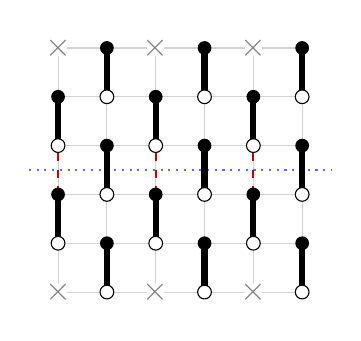
\begin{tikzpicture}[scale=0.62]
  \draw[gray!35] (1,1) grid (6,6);
  \draw[blue!60, dotted, thick] (0.4,3.5) -- (6.6,3.5);
  \foreach \x in {2,4,6} \foreach \y in {1,3,5} \draw[line width=2.2pt] (\x,\y) -- (\x,\y+1);
  \foreach \x in {1,3,5} \foreach \y in {2,4} \draw[line width=2.2pt] (\x,\y) -- (\x,\y+1);
  \foreach \x in {1,3,5} \draw[red!75!black, dashed, thick] (\x,3) -- (\x,4);
  \foreach \x in {1,...,6}{
    \foreach \y in {1,...,6}{
      \pgfmathtruncatemacro{\parity}{mod(\x+\y,2)}
      \ifnum\parity=0 \fill (\x,\y) circle (4pt); \else \draw[fill=white] (\x,\y) circle (4pt); \fi
    }
  }
  \foreach \x in {1,3,5}{
    \fill[white] (\x,6) circle (5pt); \node[gray] at (\x,6) {\large$\times$};
    \fill[white] (\x,1) circle (5pt); \node[gray] at (\x,1) {\large$\times$};
  }
\end{tikzpicture}
\caption{Proposition~\ref{prop:flux} for $m=6$. Crosses mark the removed boundary vertices: white vertices of the top row and black vertices of the bottom row. Thick edges form a perfect matching of the remnant. The dotted line is the middle line. The dashed edges cross it with a white upper endpoint, and no perfect matching of the remnant uses them. A computer check for all even $m\le 30$ is in \texttt{checks/lemma8\_flux.py}.}
\label{fig:flux}
\end{figure}

Boundary conditions can freeze square-lattice edges at distance $m/2$ from the patch boundary. This is the height-function rigidity of square-lattice dimers. Valiant's step of multiplying local ratios is therefore unavailable. We replace it with a global estimate. Fix a set $F$ of $t$ forbidden edges, one in each of $t$ rows spaced three apart. A tilted Kasteleyn determinant gives the identity $\E[(1-\eta)^{\abs{M\cap F}}]=\det(I-\eta H)$, where $H$ is a $t\times t$ matrix of inverse-Kasteleyn entries (Lemma~\ref{lem:tilted}). Carleman's inequality bounds this determinant using only $\tr H$, which is about $t/4$ because bulk edge marginals are near $1/4$, and $\norm{H}_F^2$. The entries of $H$ decay like $1/\abs{i-j}$, and $\sum_k k^{-2}$ converges, so $\norm{H}_F^2=O(t)$. This gives $\Pr(M\cap F=\emptyset)\le e^{-\Omega(t)}$ with no independence assumption and no local replaceability.

\subsection{Results}\label{sec:intro-results}

Section~\ref{sec:results} states the formal versions:
\begin{itemize}
\item \textbf{Theorem A} (edge profiles). For every even $L\ge264$, every split $E=A\sqcup B$ with $\abs A,\abs B\ge n/3$, and every $S\subseteq V$, the profile event $\{\prof_A(M)=S\}$ has probability at most $e^{-c(L)L}$. The function $c(L)$ is explicit and nondecreasing, with $c(400)\ge1/7980$, $c(1000)\ge1/1129$ and $c(L)\to1/(357.2361493\ldots)$
\item \textbf{Theorem A$'$} (vertex cuts). The same bound holds for the event that no edge of $M$ joins $S$ to $V\setminus S$, for every $S$ with $L^2/3\le\abs S\le 2L^2/3$.
\item \textbf{Corollary~\ref{cor:entanglement}} (min-entropy). Across every link bipartition with at least $n/3$ links on each side, the Rokhsar--Kivelson state on the free square has R\'enyi-$\infty$ entanglement entropy at least $c(L)L$.
\item \textbf{Theorem B} (robust PC lower bound). Nonnegative smooth decomposable PCs with leaves of arity at most $2n/3$ that are $\eps$-close to $U_L$ in TV have size at least $(1-\eps)^2e^{c(L)L}$.
\item \textbf{Theorem C} (upper bound). A smooth, decomposable, deterministic PC with indicator leaves computes $Z_L\cdot U_L$ exactly with size at most $3L^2(1+\sqrt2)^L+2n$. A binary, structured version has size at most $6L^2(1+\sqrt2)^L+2n$.
\item \textbf{Theorem D} (exact monotone and tropical). Every monotone arithmetic circuit for a polynomial whose monomials are exactly the perfect matchings of the grid, with any positive coefficients, has size at least $e^{c(L)L}$. Every $(\min,+)$ circuit for the minimum-weight perfect matching on nonnegative weights has the same bound. The proof goes through Theorem~A$'$, which plays the role of Valiant's Corollary~9.
\item \textbf{Signed circuits} (Section~\ref{sec:signed}). The Kasteleyn determinant gives a polynomial-size generating circuit for $U_L$ that uses subtraction. Known conversions \cite{AgarwalBlaser24,BroadrickZhangVdB24} turn it into a polynomial-size signed circuit for the network polynomial, but that circuit is not syntactically decomposable. For signed \emph{structured}-decomposable circuits with univariate leaves, exact representation needs size at least $e^{c(L)L}-1$ (Proposition~\ref{prop:structured-signed}). For signed unstructured decomposable circuits with univariate leaves the question is open.
\end{itemize}

\begin{table}[t]
\centering
\small
\begin{tabular}{@{}p{5.6cm}p{2.7cm}p{2.9cm}p{2.4cm}@{}}
\toprule
Model (target $P_L$, $\OPT_L$ or $U_L$) & lower bound & upper bound & where\\
\midrule
monotone arithmetic circuit for $P_L$ & $e^{c(L)L}$ & $O(L^2(1+\sqrt2)^L)$ & Thm D, C\\
$(\min,+)$ circuit for $\OPT_L$, weights $\ge0$ & $e^{c(L)L}$ & $O(L^2(1+\sqrt2)^L)$ & Thm D, C\\
nonnegative smooth decomposable PC, leaf arity $\le2n/3$, TV $\le\eps$ & $(1-\eps)^2e^{c(L)L}$ & $O(L^2(1+\sqrt2)^L)$ & Thm B, C\\
signed structured-decomposable, univariate leaves, exact & $e^{c(L)L}-1$ & $O(L^2(1+\sqrt2)^L)$ & Prop \ref{prop:structured-signed}, Thm C\\
signed decomposable (unstructured), univariate leaves & \textbf{open} & $O(L^2(1+\sqrt2)^L)$ & Sec.~\ref{sec:signed}\\
signed circuit for the generating polynomial (PGC) & --- & $\mathrm{poly}(n)$ & Sec.~\ref{sec:signed}\\
\bottomrule
\end{tabular}
\caption{Sizes for the square-grid targets. Here $n=2L(L-1)$, $L$ is even, and $c(L)\ge1/1129$ for $L\ge1000$. For every fixed error below one, the nonnegative PC row gives size $\exp(\Theta(L))$. The upper bound $\ln(1+\sqrt2)\approx0.881$ in the exponent and the certified lower bound $c(L)$ differ by a factor of about $10^3$.}
\label{tab:summary}
\end{table}

\subsection{What this paper does not claim}\label{sec:intro-scope}

\begin{itemize}
\item \textbf{No general separation is claimed.} Proposition~\ref{prop:triangular} and the code example of Section~\ref{sec:codes} already give constant-TV separations between nonnegative decomposable PCs and models with efficient exact inference. The code example even gives $\exp(\Omega(n))$. Our results concern the square grid.
\item \textbf{This is a representation-size result.} For $U_L$, evidence probabilities, marginals, conditionals and exact samples are all computable in polynomial time with planar Kasteleyn determinants (Section~\ref{sec:signed}).
\item \textbf{The constants are crude.} The certified rate $1/1129$ at $L=1000$ is about 100 times smaller than the observed decay rate along the same forbidden sets (Section~\ref{sec:constants}). The bounds say nothing explicit for $L<264$.
\item \textbf{Scope.} We cover the free square with even $L$ and edge-indicator variables. We do not cover rectangles, the torus, or other encodings such as vertex-partner variables (Section~\ref{sec:open}).
\end{itemize}

\subsection{Organization}
Section~\ref{sec:prelim} fixes notation and circuit models. Section~\ref{sec:results} states Theorems~A and~A$'$ and the entanglement corollary. Sections~\ref{sec:kasteleyn}--\ref{sec:selection} prove them: Kasteleyn algebra and Carleman's inequality, the free-square kernel bound, and the selection lemmas with explicit constants. Section~\ref{sec:circuits} derives the circuit lower bounds (Theorems~B and~D and Proposition~\ref{prop:triangular}). Section~\ref{sec:upper} gives the matching upper bound. Section~\ref{sec:signed} discusses signed weights. Sections~\ref{sec:related} and~\ref{sec:open} cover related work and open problems. Appendix~\ref{app:checks} lists the numerical checks.

\section{Preliminaries}\label{sec:prelim}

\paragraph{The grid.} Fix an even integer $L$ and put $N:=L+1$, which is odd. The grid $G_L$ has vertex set $V=\{1,\dots,L\}^2$. We call $x_1$ the column and $x_2$ the row of $x=(x_1,x_2)$. Edges join vertices at Euclidean distance one. There are $n:=2L(L-1)$ edges. A vertex is \emph{black} if $x_1+x_2$ is even and \emph{white} otherwise, so each colour class has $L^2/2$ vertices and every edge joins a black vertex to a white one. We write $\PM_L$ for the set of perfect matchings (domino tilings), $Z_L:=\abs{\PM_L}$, and identify $M\in\PM_L$ with its indicator vector in $\{0,1\}^E$. $U_L$ is the uniform distribution on $\PM_L$, viewed as a distribution on $\{0,1\}^n$. For odd $L$ there are no perfect matchings, so evenness is part of the definition of $U_L$, not a proof convenience.

The \emph{boundary distance} of $x\in V$ is $\min(x_1,N-x_1,x_2,N-x_2)$. For $x,y\in V$ we set $D(x,y)$ to be the smaller boundary distance of $x$ and $y$, and for an edge $e=\{x,y\}$ we set $D(e):=D(x,y)$.

\paragraph{Cuts and profiles.} A \emph{balanced edge cut} is a partition $E=A\sqcup B$ with $\abs A,\abs B\ge n/3$. For a matching $M$ and $A\subseteq E$, the \emph{$A$-profile} is
\[
  \prof_A(M):=\{v\in V:\ \text{the edge of $M$ at $v$ lies in $A$}\}.
\]
Let $R_{A,S}:=\{M\in\PM_L:\prof_A(M)=S\}$ and
\[
  \alpha_L:=\max\bigl\{U_L(R_{A,S}) : A\sqcup B \text{ a balanced edge cut},\ S\subseteq V\bigr\}.
\]
For $S\subseteq V$, let $\cA_S$ be the set of subsets of $A$ that perfectly match $S$, and $\cB_S$ the set of subsets of $B$ that perfectly match $V\setminus S$. Then
\begin{equation}\label{eq:rectangle}
  R_{A,S}=\{\alpha\cup\beta:\ \alpha\in\cA_S,\ \beta\in\cB_S\},
\end{equation}
and the map $(\alpha,\beta)\mapsto\alpha\cup\beta$ is a bijection from $\cA_S\times\cB_S$ onto $R_{A,S}$. Indeed, every such union is a perfect matching with profile $S$, and every perfect matching with profile $S$ splits this way. The sets $\cA_S$ are pairwise disjoint for distinct $S$, since an edge set determines the vertices it covers. The same holds for the $\cB_S$.

A \emph{balanced vertex set} is an $S\subseteq V$ with $L^2/3\le\abs S\le 2L^2/3$. Write
\[
  \mathrm{Cut}(S):=\{M\in\PM_L:\ \text{no edge of $M$ joins $S$ to $V\setminus S$}\},\qquad
  \beta_L:=\max_{S\ \text{balanced}} U_L(\mathrm{Cut}(S)).
\]
If $A\sqcup B$ is any edge partition, then $R_{A,S}\subseteq\mathrm{Cut}(S)$, but $S$ need not be balanced. So neither $\alpha_L$ nor $\beta_L$ controls the other directly.

\paragraph{Distances between distributions.} For distributions $P,Q$ on a finite set, $\TV(P,Q)=\frac12\sum_x\abs{P(x)-Q(x)}$, so $1-\TV(P,Q)=\sum_x\min(P(x),Q(x))$. The Bhattacharyya coefficient is $\BC(P,Q)=\sum_x\sqrt{P(x)Q(x)}$. The same formulas define $\BC(P,Q)$ when $Q$ is a nonnegative function of total mass at most one.

\subsection{Circuit models}\label{sec:models}

\paragraph{Probabilistic circuits.} A \emph{probabilistic circuit} (PC) over $x\in\{0,1\}^n$ is a directed acyclic graph with one root and three kinds of node.
\begin{itemize}
\item \emph{Leaves} are nonnegative functions of at most $r$ of the variables. The \emph{arity} is $r$; \emph{univariate} means $r=1$. Indicator leaves $[x_e=0]$ and $[x_e=1]$ are the usual choice.
\item \emph{Sum nodes} take a weighted sum of their children. Here the weights are nonnegative.
\item \emph{Product nodes} multiply their children.
\end{itemize}
The \emph{scope} $X_v$ of a node $v$ is the set of variables appearing in leaves below $v$. Node $v$ computes a function $f_v$ of $x_{X_v}$. The circuit computes $f_C:=f_{\mathrm{root}}\ge0$ and represents the distribution $Q_C:=f_C/\sum_xf_C(x)$. The circuit is \emph{decomposable} if the children of each product node have pairwise disjoint scopes. It is \emph{smooth} if the children of each sum node have equal scopes. It is \emph{deterministic} if, for each sum node, the children's supports are pairwise disjoint. It is \emph{structured-decomposable} (with respect to a vtree, a rooted binary tree whose leaves are the variables) if every product node is binary and has a vtree node whose left and right variable sets contain the scopes of its two children. The size $\abs C$ is the number of nodes plus the number of wires. Unless stated otherwise, we assume neither determinism nor structure.

A \emph{signed} circuit has the same syntax but allows arbitrary real sum weights and real-valued leaves.

\paragraph{Arithmetic and tropical circuits.} A \emph{monotone arithmetic circuit} has binary $+$ and $\times$ gates, inputs $z_e$ ($e\in E$) and nonnegative real constants. It computes a formal polynomial; we do not identify $z_e^2$ with $z_e$. Its size is the number of nodes (gates, inputs and constants). For unbounded fan-in, count wires instead; this changes sizes by at most a factor of two. A $(\min,+)$ circuit has binary $\min$ and $+$ gates, inputs $w_e$, and constants in $\R\cup\{+\infty\}$. We write
\[
  P_L(z):=\sum_{M\in\PM_L}\prod_{e\in M}z_e,\qquad \OPT_L(w):=\min_{M\in\PM_L}\sum_{e\in M}w_e .
\]
\paragraph{Generating circuits.} The \emph{generating polynomial} of a distribution $Q$ on $\{0,1\}^n$ is $\sum_xQ(x)\prod_{e:x_e=1}z_e$. A \emph{probabilistic generating circuit} (PGC)~\cite{ZhangJubaVdB21} is an arithmetic circuit, with subtraction allowed, that computes it.

\section{Main results}\label{sec:results}

Throughout, $A_\star:=\frac{1+\sqrt2}{2\ln(1+\sqrt2)}\approx1.369574$ is the kernel constant of Section~\ref{sec:kernel}. The function $c(L)$ is defined in~\eqref{eq:cL}. It is positive and nondecreasing for even $L\ge264$, and
\begin{gather*}
  c(264)\ge 1/(7.76\cdot10^{7}),\qquad c(400)\ge1/7980,\qquad c(1000)\ge1/1129,\\
  c(10^4)\ge1/411,\qquad \lim_{L\to\infty}c(L)=1/(357.2361493\ldots)
\end{gather*}
The finite-$L$ inequalities are certified by exact rational bounds. The displayed limit is a numerical evaluation of the defining series, not the conservative certificate (Section~\ref{sec:constants}).

\begin{named}{Theorem A (edge profiles)}
Let $L\ge264$ be even. For every balanced edge cut $A\sqcup B$ and every $S\subseteq V$,
\[
  U_L\bigl(\prof_A(M)=S\bigr)\le e^{-c(L)L}.
\]
That is, $\alpha_L\le e^{-c(L)L}$.
\end{named}

\begin{named}{Theorem A$'$ (vertex cuts)}
Let $L\ge264$ be even. For every $S\subseteq V$ with $L^2/3\le\abs S\le 2L^2/3$,
\[
  U_L\bigl(\text{no edge of $M$ joins $S$ to $V\setminus S$}\bigr)\le e^{-c(L)L}.
\]
That is, $\beta_L\le e^{-c(L)L}$.
\end{named}

The two statements are incomparable (Section~\ref{sec:prelim}). Theorem~A is the one that controls arbitrary, possibly interlaced, edge partitions. Theorem~A$'$ is the one that controls monotone circuits, whose balanced products split the vertex set but not necessarily the edge set (Section~\ref{sec:monotone}). Both follow from one estimate: the probability of avoiding a row-spread set of $t$ bulk edges is at most $e^{-\Omega(t)}$ (Proposition~\ref{prop:avoid}).

\subsection{Min-entropy of the Rokhsar--Kivelson state}

Put one qubit on each link $e\in E$, with $\ket1$ meaning ``dimer on $e$''. The Rokhsar--Kivelson (RK) state on the free square is the equal-amplitude superposition of all dimer coverings,
\[
  \ket{\Psi_L}:=Z_L^{-1/2}\sum_{M\in\PM_L}\ket M,\qquad \ket M:=\bigotimes_{e\in E}\ket{\one[e\in M]} .
\]
It is the ground state of the quantum dimer model at the RK point~\cite{RokhsarKivelson88}. Measuring $\ket{\Psi_L}$ in the dimer basis gives a sample from $U_L$.

\begin{definition}
Let $\rho$ be a density matrix with largest eigenvalue $\lambda_{\max}(\rho)$. Its \emph{min-entropy} (R\'enyi-$\infty$ entropy) is $S_\infty(\rho):=-\ln\lambda_{\max}(\rho)$. For a pure state $\ket\Psi$ on $\mathcal H_A\otimes\mathcal H_B$ with reduced state $\rho_A=\tr_B\ket\Psi\bra\Psi$, the operational \emph{single-copy entanglement} is $E_1=\ln\lfloor1/\lambda_{\max}(\rho_A)\rfloor$~\cite{EisertCramer05}. Since R\'enyi entropies are nonincreasing in their order, $S_\infty(\rho_A)\le S_\alpha(\rho_A)$ for every $\alpha\in[0,\infty]$, including the von Neumann entropy $S_1$.
\end{definition}

\begin{corollary}[min-entropy for every balanced link bipartition]\label{cor:entanglement}
Let $L\ge264$ be even. Split the links into $E=A\sqcup B$ with $\abs A,\abs B\ge n/3$, and let $\rho_A$ be the reduced state of $\ket{\Psi_L}$ on the qubits in $A$. Then
\[
  S_\infty(\rho_A)\ \ge\ c(L)\,L ,
\]
and hence $S_\alpha(\rho_A)\ge c(L)L$ for every R\'enyi order $\alpha$. Operationally,
\[
  E_1\ge\ln\lfloor\exp(c(L)L)\rfloor\ge c(L)L-\ln2.
\]
\end{corollary}

\begin{proof}
Group the dimer coverings by their $A$-profile. By~\eqref{eq:rectangle},
\[
  \ket{\Psi_L}=\sum_S\sqrt{p_S}\,\ket{a_S}\otimes\ket{b_S},\qquad
  \ket{a_S}=\abs{\cA_S}^{-1/2}\sum_{\alpha\in\cA_S}\ket\alpha,\quad
  \ket{b_S}=\abs{\cB_S}^{-1/2}\sum_{\beta\in\cB_S}\ket\beta,
\]
with $p_S=\abs{\cA_S}\abs{\cB_S}/Z_L=U_L(R_{A,S})$. The sum runs over the profiles $S$ for which both sets are nonempty. Vectors $\ket{a_S}$ with distinct $S$ are supported on disjoint sets of basis states, so they are orthonormal, and likewise the $\ket{b_S}$. So this is a Schmidt decomposition, and the eigenvalues of $\rho_A$ are the numbers $p_S$. Theorem~A gives $\max_Sp_S\le e^{-c(L)L}$.
\end{proof}

The bound is linear in $L$, the length of a straight cut through the square, and it holds for every balanced link bipartition. That includes disconnected, interlaced and fractal-looking ones. We do not claim a matching upper bound for arbitrary partitions. A bound of order $L$ for the von Neumann entropy alone would not imply the corollary: a distribution can have one heavy atom and large Shannon entropy. Stéphan, Misguich and Pasquier~\cite{StephanMisguichPasquier12} relate R\'enyi entropies of RK states to classical boundary probabilities and study cylinder and Kitaev--Preskill geometries. We are not aware of a statement over all link bipartitions of the free square (see Section~\ref{sec:related-physics}).

\subsection{Circuit consequences}

\begin{named}{Theorem B (nonnegative decomposable PCs, constant TV)}
Let $L\ge264$ be even. Let $C$ be a smooth decomposable PC with nonnegative weights and leaves of arity at most $2n/3$. If $\TV(U_L,Q_C)\le\eps$, then
\[
  \abs C\ \ge\ \frac{(1-\eps)^2}{\alpha_L}\ \ge\ (1-\eps)^2e^{c(L)L}.
\]
Determinism and structure are not assumed. If $C$ is decomposable but not smooth, smoothing costs a factor $O(n)$ in size, so $\abs C\ge\Omega((1-\eps)^2e^{c(L)L}/n)$.
\end{named}

\begin{named}{Theorem C (matching upper bound)}
For even $L\ge4$ there is a smooth, decomposable, deterministic PC with univariate indicator leaves and all weights equal to one, of size at most $3L^2(1+\sqrt2)^L+2n$, that computes $Z_L\cdot U_L$ exactly. Splitting its products into binary ones makes it also structured-decomposable, with size at most $6L^2(1+\sqrt2)^L+2n$. The same construction gives a monotone arithmetic circuit for $P_L$ and a $(\min,+)$ circuit for $\OPT_L$, each of size $O(L^2(1+\sqrt2)^L)$.
\end{named}

So for nonnegative smooth decomposable PCs with leaves of arity at most $2n/3$, the minimum size needed to represent $U_L$ is $\exp(\Theta(L))=\exp(\Theta(\sqrt n))$, exactly and for every fixed error below one, with or without determinism.

\begin{named}{Theorem D (exact monotone and tropical circuits)}
Let $L\ge264$ be even.
\begin{enumerate}[label=(\roman*)]
\item Let $F$ be any polynomial whose monomials are exactly $\{\prod_{e\in M}z_e:M\in\PM_L\}$, with arbitrary positive coefficients. Every monotone arithmetic circuit for $F$ has at least $1/\beta_L\ge e^{c(L)L}$ gates.
\item Every $(\min,+)$ circuit that computes $\OPT_L(w)$ for all $w\in\R_{\ge0}^E$ has at least $e^{c(L)L}$ gates. This holds for any finite real constants and $+\infty$ in the circuit.
\end{enumerate}
\end{named}

Theorem~C shows that (i) is tight up to the constant in the exponent for $F=P_L$, and for coefficients that factor over edges. For general positive coefficients it is not tight: if the $Z_L$ coefficients are algebraically independent, a circuit with $q$ constants has transcendence degree at most $q$, so it needs at least $Z_L\ge2^{L^2/4}$ constants. We include (i) for all positive coefficients because it shows that the bound comes from the support alone.

\begin{remark}[how Theorem D is proved, and what Theorem A does not give]\label{rem:K5-route}
A monotone circuit for $F$ yields a sum of at most $s$ products $g_jh_j$ whose degrees are balanced (Lemma~\ref{lem:degree-decomp}). Each product covers a balanced vertex set but may use far fewer than $n/3$ edge variables on one side, since $\deg g_j>L^2/6$ only forces $\abs{\vars(g_j)}>L^2/6\approx n/12$. So Theorem~A does not apply directly. We use Theorem~A$'$ instead. It is proved by the same method as Theorem~A, with a selection lemma for vertex cuts (Lemma~\ref{lem:select-vertex}) in place of the one for edge cuts. Our first proof of Theorem~D went through a combinatorial block measure and gave a constant near $3\cdot10^{-13}$ for $4\mid L$. We do not include it.
\end{remark}

\subsection{Scope of the hypotheses}\label{sec:scope}

\begin{itemize}
\item \textbf{Decomposability is needed.} Without it the claim of Theorem~B is false, even with nonnegative weights and univariate leaves: $Z_LU_L(x)=\prod_{v\in V}\sum_{e\ni v}\bigl([x_e=1]\prod_{e'\ni v,\,e'\ne e}[x_{e'}=0]\bigr)$ is a circuit of size $O(n)$. It is not decomposable, because each edge variable appears in two vertex factors, and marginals cannot be read off by evaluating it.
\item \textbf{Leaf arity is needed.} One leaf of arity $n$ can be $U_L$. A leaf of arity $n-1$ already defeats any fixed $\eps$ above about $1/4$. Take $Q=U_L^{(-e)}\otimes\delta_0$ for a bulk edge $e$, where $U_L^{(-e)}$ is the marginal on the other edges. Then $\TV(U_L,Q)=\Pr(e\in M)\approx1/4$. Our proof allows any arity up to $2n/3$, with each leaf counted as one node.
\item \textbf{Smoothness is technical.} Multiply each child of a sum node by constant-one leaves $[x=0]+[x=1]$ for its missing variables. This costs a factor $O(n)$.
\item \textbf{Nonnegative weights.} The proofs of Theorems~B and~D use nonnegativity in two places: in the overlap inequality $\sqrt{\sum_ua_u}\le\sum_u\sqrt{a_u}$ for nonnegative mixture weights, and in the claim that every product term is supported on perfect matchings. Section~\ref{sec:signed} discusses signed circuits.
\item \textbf{The error measure.} The bound is $(1-\eps)^2e^{c(L)L}$. It stays superpolynomial while $1-\eps\ge e^{-o(L)}$, and says nothing at $\eps=1$.
\end{itemize}

\section{Kasteleyn algebra and Carleman's inequality}\label{sec:kasteleyn}

\subsection{Kasteleyn matrices and the common phase}

Let $\mathsf B$ and $\mathsf W$ be the sets of black and white vertices. The \emph{complex Kasteleyn matrix} $K$ is the $\mathsf B\times\mathsf W$ matrix with
\[
  K(b,w)=\begin{cases}1 & \text{if $\{b,w\}$ is a horizontal edge,}\\ i & \text{if $\{b,w\}$ is a vertical edge,}\\ 0&\text{otherwise.}\end{cases}
\]
For edge weights $z\in\C^E$, let $K(z)$ have entries $K(b,w)z_{bw}$. Let $T$ be the symmetric $V\times V$ matrix with $T(b,w)=T(w,b)=K(b,w)$ and zero entries between vertices of the same colour. Writing $P_L$ for the adjacency matrix of the path $1-2-\dots-L$ (no confusion with the polynomial $P_L$ will arise), we have
\begin{equation}\label{eq:T-tensor}
  T=P_L\otimes I+i\,I\otimes P_L ,
\end{equation}
where the first factor acts on columns and the second on rows. In block form $T=\begin{psmallmatrix}0&K\\K^{\top}&0\end{psmallmatrix}$, so $T^{-1}(w,b)=K^{-1}(w,b)$ for $w\in\mathsf W$, $b\in\mathsf B$. We show in Section~\ref{sec:kernel-diag} that $T$, and hence $K$, is invertible.

The \emph{real gauge} is $K':=D_{\mathsf B}KD_{\mathsf W}$ with diagonal matrices $D_{\mathsf B}(b)=(-i)^{b_2}$ and $D_{\mathsf W}(w)=i^{w_2}$.

\begin{lemma}[face signs]\label{lem:faces}
$K'$ has entries in $\{0,\pm1\}$. A horizontal edge has $K'(b,w)=+1$. A vertical edge has $K'(b,w)=-1$ if the white endpoint lies above the black one, and $+1$ if it lies below. For every unit square of the grid, the product of the four entries of $K'$ on its sides is $-1$.
\end{lemma}

\begin{proof}
For a horizontal edge $b_2=w_2$, so $K'(b,w)=(-i)^{b_2}\cdot1\cdot i^{b_2}=1$. For a vertical edge with $w_2=b_2+1$ we get $(-i)^{b_2}\cdot i\cdot i^{b_2+1}=i^2=-1$. With $w_2=b_2-1$ we get $(-i)^{b_2}\cdot i\cdot i^{b_2-1}=1$. Take a unit square with lower-left corner $(x_1,x_2)$. Both horizontal sides give $+1$. If $(x_1,x_2)$ is black, the left side has white above black ($-1$) and the right side has white below black ($+1$). If $(x_1,x_2)$ is white, the two signs swap. Either way the product is $-1$.
\end{proof}

The next lemma is Kasteleyn's theorem~\cite{Kasteleyn61} for the square grid. We include the standard proof because the tilted identity below depends on it.

\begin{lemma}[common phase]\label{lem:common-phase}
All perfect matchings contribute the same sign to $\det K'$. Hence there are $\epsilon_L\in\{\pm1\}$ and a constant $\omega_L\in\C$ with $\abs{\omega_L}=1$ such that, as polynomials in $z$,
\begin{equation}\label{eq:kasteleyn}
  \det K'(z)=\epsilon_L\,P_L(z),\qquad \det K(z)=\omega_L\,P_L(z).
\end{equation}
In particular $\abs{\det K}=Z_L$.
\end{lemma}

\begin{proof}
Fix orderings of $\mathsf B$ and $\mathsf W$. A nonzero term of the Leibniz expansion of $\det K'(z)$ is $\sgn(\sigma)\prod_bK'(b,\sigma(b))z_{b\sigma(b)}$ for a bijection $\sigma:\mathsf B\to\mathsf W$ whose pairs $\{b,\sigma(b)\}$ form a perfect matching $M_\sigma$. Distinct matchings give distinct monomials. So it suffices to show that the sign $\tau(M):=\sgn(\sigma_M)\prod_{e\in M}K'(e)$ is the same for all $M$.

Let $M,M'$ be perfect matchings. The symmetric difference $M\triangle M'$ is a disjoint union of simple cycles $C_1,\dots,C_q$ that alternate between $M$ and $M'$. If $C_j$ has length $2\ell_j$, then $\sigma_{M'}\sigma_M^{-1}$ restricted to the white vertices of $C_j$ is an $\ell_j$-cycle, with sign $(-1)^{\ell_j-1}$. Edges of $M\cap M'$ cancel in the ratio. Since entries are $\pm1$,
\[
  \tau(M)\tau(M')=\prod_{j=1}^q(-1)^{\ell_j-1}\prod_{e\in C_j}K'(e).
\]
We claim that $\prod_{e\in C}K'(e)=(-1)^{\ell+1}$ for each such cycle $C$ of length $2\ell$, which makes every factor equal to $+1$.

The cycle $C$ is a simple closed lattice curve. The grid vertices, edges and unit squares inside it form a connected plane graph whose outer boundary is $C$. Let $p$ be the number of vertices strictly inside $C$, $E_{\mathrm{in}}$ the number of edges strictly inside, and $f$ the number of unit squares inside. Each unit square has sign product $-1=(-1)^{2+1}$ by Lemma~\ref{lem:faces}. Multiplying over the $f$ squares inside, each interior edge appears twice and each edge of $C$ once, so
\[
  \prod_{e\in C}K'(e)=(-1)^f .
\]
Euler's formula for the plane graph inside $C$ (with $f$ bounded faces) gives $(2\ell+p)-(2\ell+E_{\mathrm{in}})+f=1$, so $f=1+E_{\mathrm{in}}-p$. Counting edge--face incidences gives $4f=2\ell+2E_{\mathrm{in}}$, so $E_{\mathrm{in}}=2f-\ell$. Substituting, $f=1+2f-\ell-p$, hence $f=\ell+p-1$ and
\[
  \prod_{e\in C}K'(e)=(-1)^{\ell+p+1}.
\]
Finally $p$ is even. A vertex strictly inside $C$ is matched by $M$ to a neighbour that is inside $C$ or on $C$. Every vertex of $C$ is matched by $M$ along $C$, because $C$ alternates between $M$ and $M'$. So $M$ matches the interior vertices among themselves. This proves the claim and the first identity in~\eqref{eq:kasteleyn}. The second follows from $K(z)=D_{\mathsf B}^{-1}K'(z)D_{\mathsf W}^{-1}$, with $\omega_L=\epsilon_L/(\det D_{\mathsf B}\det D_{\mathsf W})$.
\end{proof}

The identity~\eqref{eq:kasteleyn} was also checked exactly for $L=2,4,6$ (Appendix~\ref{app:checks}). All $1$, $9$ and $25$ unit squares have sign product $-1$. The common real sign over all $2$, $36$ and $6728$ matchings is $+1$ in the script's orderings. The polynomial identity holds in integer arithmetic at six random integer points per $L$, half of which have negative entries.

\subsection{The tilted identity}

\begin{lemma}[tilted identity]\label{lem:tilted}
Let $F=\{e_1,\dots,e_t\}$ be distinct edges with $e_j=\{b_j,w_j\}$, $b_j$ black, and put $\kappa_j:=K(b_j,w_j)$. Define the $t\times t$ matrix
\[
  H_{ij}:=K^{-1}(w_i,b_j)\,\kappa_j .
\]
Then for every $\eta\in[0,1]$,
\[
  \det(I-\eta H)=\E_{U_L}\bigl[(1-\eta)^{\abs{M\cap F}}\bigr]\in[0,1].
\]
In particular $\det(I-\eta H)$ is real, $\det(I-\eta H)\ge U_L(M\cap F=\emptyset)$, and $H_{jj}=U_L(e_j\in M)$.
\end{lemma}

\begin{proof}
Let $K_\eta$ be $K$ with the entries on $F$ multiplied by $1-\eta$. With $U$ the $\mathsf B\times t$ matrix whose $j$-th column is $\kappa_j\one_{b_j}$, and $V$ the $\mathsf W\times t$ matrix whose $j$-th column is $\one_{w_j}$, we have $K_\eta=K-\eta UV^{\top}$, because the edges are distinct. By~\eqref{eq:kasteleyn}, evaluated at $z_e=1-\eta$ on $F$ and $z_e=1$ elsewhere,
\[
  \frac{\det K_\eta}{\det K}=\frac{\omega_L\sum_M(1-\eta)^{\abs{M\cap F}}}{\omega_LZ_L}=\E\bigl[(1-\eta)^{\abs{M\cap F}}\bigr].
\]
By the matrix determinant lemma, $\det(K-\eta UV^{\top})=\det K\cdot\det(I_t-\eta V^{\top}K^{-1}U)$, and $(V^{\top}K^{-1}U)_{ij}=K^{-1}(w_i,b_j)\kappa_j=H_{ij}$. The case $t=1$ gives $1-\eta H_{11}=1-\eta\Pr(e_1\in M)$. Finally $(1-\eta)^{\abs{M\cap F}}\ge\one[M\cap F=\emptyset]$.
\end{proof}

Changing to the real gauge conjugates $H$ by a diagonal unitary matrix. This changes neither the determinant nor the moduli of the entries. Lemma~\ref{lem:tilted} was checked in exact rational arithmetic against enumeration for $25$ random sets $F$ with $\abs F\le8$ at each $L\in\{2,4,6\}$, with $\eta=2/5$ (Appendix~\ref{app:checks}).

\subsection{Carleman's inequality and avoidance}

\begin{lemma}[Carleman-type determinant bound]\label{lem:carleman}
For every complex $t\times t$ matrix $X$,
\[
  \abs{\det(I-X)}\le\exp\Bigl(-\mathrm{Re}\tr X+\tfrac12\norm X_F^2\Bigr),
\]
where $\norm X_F$ is the Frobenius (Hilbert--Schmidt) norm.
\end{lemma}

\begin{proof}
If $I-X$ is singular there is nothing to prove. Otherwise let $\sigma_1,\dots,\sigma_t>0$ be its singular values. Using $\ln u\le u-1$ with $u=\sigma_k^2$,
\[
  2\ln\abs{\det(I-X)}=\sum_k\ln\sigma_k^2\le\sum_k(\sigma_k^2-1)=\tr\bigl((I-X)^*(I-X)\bigr)-t=-2\,\mathrm{Re}\tr X+\norm X_F^2. \qedhere
\]
\end{proof}

This is the finite-dimensional case of Carleman's inequality $\abs{\det_2(I+Y)}\le\exp(\frac12\norm Y_F^2)$ for the regularized determinant $\det_2(I+Y)=\det(I+Y)e^{-\tr Y}$, with $Y=-X$. Inequalities of this type go back to Carleman~\cite{Carleman21}; Simon~\cite[Ch.~9]{Simon05} treats regularized determinants. We use only the statement proved above.

\begin{proposition}[avoidance]\label{prop:avoid}
Let $F$ and $H$ be as in Lemma~\ref{lem:tilted}. Suppose $\tr H\ge pt$ and $\norm H_F^2\le Rt$ with $0<p\le R$. Then
\[
  U_L(M\cap F=\emptyset)\le\exp\Bigl(-\frac{tp^2}{2R}\Bigr).
\]
\end{proposition}

\begin{proof}
Take $\eta=p/R\in(0,1]$. The trace $\tr H=\sum_j\Pr(e_j\in M)$ is real. By Lemmas~\ref{lem:tilted} and~\ref{lem:carleman},
\[
  U_L(M\cap F=\emptyset)\le\det(I-\eta H)\le\exp\bigl(-\eta tp+\tfrac12\eta^2tR\bigr)=\exp\Bigl(-\frac{tp^2}{2R}\Bigr).\qedhere
\]
\end{proof}

No Hermitian structure, operator-norm bound or negative dependence is used. The matrix $H$ is not Hermitian in general.

\section{The free-square kernel}\label{sec:kernel}

This section proves that $\abs{K^{-1}(w,b)}\le 4A_\star/\norm{w-b}_\infty$ for all white $w$ and black $b$, with no restriction to the bulk and no $1/L$ term. It also proves that bulk edge marginals are $1/4+O(1/D(e))$. The proof uses odd reflections onto a torus of side $2N$ and a closed form for a one-dimensional resolvent.

\paragraph{Notation.} Put $M:=2N=2(L+1)$, $c_j:=\cos(\pi j/N)$ for $j\in\Z$, $\kappa:=\asinh1=\ln(1+\sqrt2)$, and
\[
  A_\star:=\frac{1+\sqrt2}{2\kappa}\approx1.3695745,\qquad G(d):=\min\Bigl(\frac1{\sqrt2},\frac{A_\star}{d}\Bigr)\quad(d>0).
\]
The function $G$ is nonincreasing. On $\Z_M$ let $d(\cdot)$ denote cyclic distance to $0$, and for $z\in\Z_M^2$ put $\norm z_T:=\max(d(z_1),d(z_2))$.

\subsection{Diagonalization}\label{sec:kernel-diag}

The path adjacency matrix $P_L$ has orthonormal eigenvectors $\phi_j(x)=\sqrt{2/N}\sin(\pi jx/N)$ with eigenvalues $2c_j$, for $j=1,\dots,L$. By~\eqref{eq:T-tensor}, $T$ has eigenvalues $\lambda_{jk}=2c_j+2ic_k$, $1\le j,k\le L$. If $\lambda_{jk}=0$ then $c_j=c_k=0$, so $j=N/2$, which is impossible because $N$ is odd. Hence $T$ and $K$ are invertible.

Let $T_M$ be the nearest-neighbour operator on the torus $\Z_M^2$ with weight $1$ on horizontal and $i$ on vertical bonds. Its eigenfunctions are $e^{i\pi(jz_1+kz_2)/N}$ with eigenvalues $\lambda_{jk}$, $j,k\in\Z_M$. These are nonzero for the same reason. Its inverse kernel is
\[
  g(z):=M^{-2}\sum_{j,k\in\Z_M}\frac{e^{i\pi(jz_1+kz_2)/N}}{\lambda_{jk}},\qquad T_Mg=\delta_0 .
\]
Since $c_{-j}=c_j$, the function $g$ is even in each coordinate separately.

\subsection{Exact images}

\begin{lemma}[images]\label{lem:images}
For $x,y\in\{1,\dots,L\}^2$,
\[
  T^{-1}(x,y)=\sum_{\sigma\in\{\pm1\}^2}\sigma_1\sigma_2\,g(x_1-\sigma_1y_1,\ x_2-\sigma_2y_2),
\]
with indices taken mod $M$.
\end{lemma}

\begin{proof}
Let $u(x)$ be the right-hand side for $x\in\Z_M^2$. By translation invariance, $T_Mu=\sum_\sigma\sigma_1\sigma_2\delta_{(\sigma_1y_1,\sigma_2y_2)}$. Since $g$ is even in its first coordinate, substituting $\sigma_1\to-\sigma_1$ gives $u(-x_1,x_2)=-u(x_1,x_2)$. Hence $u(0,\cdot)=0$, and $u(N,\cdot)=u(-N,\cdot)=-u(N,\cdot)=0$. The same holds in the second coordinate. For $x$ in the box $\{1,\dots,N-1\}^2$, all torus neighbours of $x$ lie in $\{0,\dots,N\}^2$, and $u$ vanishes on the lines with a coordinate equal to $0$ or $N$. So $(T\,u|_{\mathrm{box}})(x)=(T_Mu)(x)$. The three reflected sources have a coordinate in $\{N+1,\dots,2N-1\}$, outside the box, so $(T_Mu)(x)=\delta_y(x)$. Since $T$ is invertible, $u|_{\mathrm{box}}=T^{-1}(\cdot,y)$.
\end{proof}

\subsection{A one-dimensional resolvent}

\begin{lemma}[1D resolvent]\label{lem:resolvent}
Let $P_M$ be the adjacency matrix of the cycle $\Z_M$, let $c\in[-1,1]\setminus\{0\}$, $\zeta\in\{2ic,-2ic\}$ and $s:=\asinh\abs c$. Then $P_M-\zeta$ is invertible, and for $x\in\Z_M$ with $d(x)=\delta\in[0,N]$,
\[
  \abs{(P_M-\zeta)^{-1}(x,0)}\le\frac{\cosh(s(N-\delta))}{2\cosh(s)\sinh(sN)} .
\]
\end{lemma}

\begin{proof}
Take $\zeta=2ic$; the other case is the same with $\mu$ replaced by $-\mu$. Put $\mu:=i\bigl(c-\sgn(c)\sqrt{1+c^2}\bigr)$. Then $\mu+\mu^{-1}=\zeta$ and $\abs\mu=\sqrt{1+c^2}-\abs c=e^{-s}<1$, since $\sinh s=\abs c$ and $\cosh s=\sqrt{1+c^2}$. On $\Z$, the function $u(x)=\mu^{\abs x+1}/(\mu^2-1)$ satisfies $u(x+1)+u(x-1)-\zeta u(x)=\delta_0(x)$. For $x\ne0$ this is $\mu+\mu^{-1}=\zeta$. At $x=0$ it reads $\frac{\mu}{\mu^2-1}(2\mu-\zeta)=\frac{\mu}{\mu^2-1}(\mu-\mu^{-1})=1$. The periodization $\sum_{\ell\in\Z}u(x+\ell M)$ converges absolutely and solves the equation on the cycle. It is the inverse kernel, because $P_M-\zeta$ has eigenvalues $2\cos(\pi k/N)-\zeta\ne0$ (a real number minus a nonzero imaginary one). Since $\mu^2=-e^{-2s}$, we have $\abs{\mu^2-1}=1+e^{-2s}$ and $\abs{u(x)}=e^{-s\abs x}/(2\cosh s)$. Finally, for a representative $x=\delta\in[0,N]$,
\[
  \sum_{\ell\in\Z}e^{-s\abs{\delta+\ell M}}=\frac{e^{-s\delta}+e^{-s(M-\delta)}}{1-e^{-sM}}=\frac{\cosh(s(N-\delta))}{\sinh(sN)} .\qedhere
\]
\end{proof}

\subsection{The torus kernel}

\begin{lemma}[torus kernel]\label{lem:torus}
\begin{enumerate}[label=(\alph*)]
\item $g(z)=0$ whenever $z_1+z_2$ is even. In particular $g(0)=0$.
\item $g(\pm e_1)=1/4$ and $g(\pm e_2)=-i/4$.
\item $\abs{g(z)}\le A_\star/\norm z_T$ for $z\ne0$.
\end{enumerate}
Consequently $\abs{g(z)}\le G(\norm z_T)$ for all $z\ne0$.
\end{lemma}

\begin{proof}
(a) Since $c_{j+N}=-c_j$, we have $\lambda_{j+N,k+N}=-\lambda_{jk}$, while the phase changes by $e^{i\pi(z_1+z_2)}=1$. The involution $(j,k)\mapsto(j+N,k+N)$ of $\Z_M^2$ has no fixed points, so $g(z)=-g(z)$.

(b) Rename the summation variables in $g(e_2)$ and use $2c_k+2ic_j=i(2c_j+2ic_{k+N})=i\lambda_{j,k+N}$. This gives $g(e_2)=-i\,g(e_1)$. By evenness $g(-e_\iota)=g(e_\iota)$. Then $(T_Mg)(0)=2g(e_1)+2i\,g(e_2)=4g(e_1)=1$.

(c) Write
\[
  g(z)=M^{-1}\sum_{j\in\Z_M}e^{i\pi jz_1/N}\Bigl[M^{-1}\sum_{k\in\Z_M}\frac{e^{i\pi kz_2/N}}{2c_j+2ic_k}\Bigr].
\]
The bracket is $(2c_j+iP_M)^{-1}(z_2,0)=-i(P_M-2ic_j)^{-1}(z_2,0)$, and $c_j\ne0$ because $N$ is odd. Summing over $j$ first instead gives the same expression with the roles of the coordinates exchanged and $(P_M+2ic_k)^{-1}(z_1,0)$ in the bracket. Apply Lemma~\ref{lem:resolvent} in a coordinate that attains $\delta:=\norm z_T\in[1,N]$. With $s_j:=\asinh\abs{c_j}$,
\[
  \abs{g(z)}\le M^{-1}\sum_{j\in\Z_M}\tau(s_j),\qquad \tau(s):=\frac{\cosh(s(N-\delta))}{2\cosh(s)\sinh(sN)} .
\]
\emph{$\tau$ is decreasing.} With $a=N-\delta<b=N$, the derivative of $\cosh(as)/\sinh(bs)$ has the sign of $a\sinh(as)\sinh(bs)-b\cosh(as)\cosh(bs)<0$, and $1/\cosh s$ is decreasing.

\emph{Lower bounds on $s_j$.} We have $\abs{c_j}=\sin(\pi\delta_j/N)$, where $\delta_j\in[0,N/2]$ is the distance from $j$ to $N/2+N\Z$. As $N$ is odd, $\delta_j\in\{\frac12,\frac32,\dots\}$. For each $m\ge0$ at most four $j\in\Z_M$ have $\delta_j=m+\frac12$, namely $N/2\pm(m+\frac12)$ and $3N/2\pm(m+\frac12)$. From $\sin x\ge2x/\pi$ on $[0,\pi/2]$ we get $\abs{c_j}\ge(2m+1)/N$. Since $\asinh$ is concave on $[0,\infty)$ with $\asinh0=0$, $\asinh y\ge\kappa y$ on $[0,1]$. Hence $s_j\ge\kappa(2m+1)/N$.

\emph{Each term.} From $\cosh(s(N-\delta))\le e^{s(N-\delta)}$, $\cosh s\ge1$ and $\sinh(sN)=\frac12e^{sN}(1-e^{-2sN})$ we get $\tau(s)\le e^{-s\delta}/(1-e^{-2sN})$. For $s\ge\kappa/N$ the denominator is at least $1-e^{-2\kappa}=1-(\sqrt2-1)^2=2(\sqrt2-1)$.

\emph{Sum.} Putting these together, with $y:=\kappa\delta/N$,
\[
  \abs{g(z)}\le\frac1{2N}\cdot4\cdot\frac{\sqrt2+1}{2}\sum_{m\ge0}e^{-(2m+1)y}=\frac{\sqrt2+1}{N}\cdot\frac{1}{2\sinh y}\le\frac{\sqrt2+1}{2\kappa\delta}=\frac{A_\star}{\delta},
\]
using $\sinh y\ge y$.

For the last claim: if $\norm z_T=1$ and $z_1+z_2$ is odd, then $z\in\{\pm e_1,\pm e_2\}$ and $\abs{g(z)}=1/4<1/\sqrt2$. If $z_1+z_2$ is even, $g(z)=0$. If $\norm z_T\ge2$ then $A_\star/\norm z_T\le A_\star/2<1/\sqrt2$.
\end{proof}

\subsection{Consequences for the free square}

\begin{proposition}[kernel bounds]\label{prop:kernel}
For all white $w$, black $b$ and edges $e$:
\begin{enumerate}[label=(\alph*)]
\item $\abs{K^{-1}(w,b)}\le4G(\norm{w-b}_\infty)\le4A_\star/\norm{w-b}_\infty$;
\item $\abs{K^{-1}(w,b)-g(w-b)}\le3G\bigl(\max(2D(w,b),\norm{w-b}_\infty)\bigr)$;
\item $\abs{\Pr(e\in M)-\frac14}\le3G(2D(e))\le\dfrac{3A_\star}{2D(e)}$.
\end{enumerate}
\end{proposition}

\begin{proof}
Use Lemma~\ref{lem:images} with $x=w$, $y=b$. The direct term $g(w-b)$ has $\norm{w-b}_T=\norm{w-b}_\infty$, because the coordinates of $w-b$ have absolute value less than $N$. Consider an image term, say with $\sigma_1=-1$. Its first coordinate $x_1+y_1$ has cyclic distance $\min(x_1+y_1,2N-x_1-y_1)$. This is at least $2\min(x_1,y_1,N-x_1,N-y_1)\ge2D(w,b)$. It is also at least $\abs{x_1-y_1}$, because $2N\ge2\max(x_1,y_1)$. The other coordinate is either reflected too, with the same bounds, or equals $x_2-y_2$. So every image term has torus norm at least $\max(2D(w,b),\norm{w-b}_\infty)\ge2$. Lemma~\ref{lem:torus} and the monotonicity of $G$ give (a) and (b). For (c), Lemma~\ref{lem:tilted} with $t=1$ gives $\Pr(e\in M)=K(b,w)K^{-1}(w,b)$. The direct term contributes $1\cdot g(\pm e_1)=1/4$ for a horizontal edge and $i\cdot g(\pm e_2)=1/4$ for a vertical edge, so (b) gives (c).
\end{proof}

Since $\norm{w-b}_\infty\ge1$, part (a) also gives $\abs{K^{-1}(w,b)}\le8A_\star/(1+\norm{w-b}_\infty)$ for \emph{all} pairs. For an edge at distance at least $\delta L$ from the boundary, $\Pr(e\in M)=\frac14+\theta\,\frac{3A_\star}{2\delta L}$ with $\abs\theta\le1$.

\begin{remark}[relation to the literature]
Inverse Kasteleyn asymptotics are classical~\cite{Kenyon97,Kenyon00,KenyonLectures}. We did not find a published statement with matching hypotheses that gives, for the ordinary free even square, a bound $C/(1+\norm{w-b})$ uniform up to the boundary together with the rate $\Pr(e\in M)=\frac14+O(1/D(e))$. Kenyon's results concern infinite-volume statistics and Temperleyan approximating domains, and a convergence theorem does not by itself give an $O(1/L)$ rate. So we prove both estimates directly. The method (sine series, odd images, a one-dimensional resolvent) is elementary and specific to the rectangle.
\end{remark}

\paragraph{Numerical checks.} Appendix~\ref{app:checks} lists them. The image formula agrees with sparse LU solves to within $5.1\cdot10^{-15}$ for $L\in\{8,16,64,128,256,300\}$, with 24 sources each, including the corners. The closed form of Lemma~\ref{lem:resolvent} matches dense inverses to $1.72\cdot10^{-15}$, and the ratio to the bound is at most $0.9988$. On the box, the observed $\sup\norm{w-b}_\infty\abs{K^{-1}(w,b)}$ grows from $1.31$ at $L=8$ to $1.66$ at $L=300$, against the proven $4A_\star=5.478$. The torus constant $A_\star$ is about $3.3$ times larger than the observed $\sup_z\norm z_T\abs{g(z)}$, which is $0.426$ at $L=8$ and $0.417$ at $L=512$. Inside the trimmed square $Q$ of Section~\ref{sec:selection}, the smallest edge marginal is $0.200$, $0.228$ and $0.237$ at $L=64$, $300$ and $512$.

\section{Selection lemmas and the proof of Theorems A and A$'$}\label{sec:selection}

Let $L\ge64$ be even, $a:=\lfloor L/32\rfloor$, and let $Q:=\{a+1,\dots,L-a\}^2$ be the trimmed square, with side $\ell:=L-2a\ge15L/16$. A \emph{row of $Q$} is a set $\{(x_1,\rho):a<x_1\le L-a\}$, and similarly for columns. An edge is \emph{inside $Q$} if both endpoints lie in $Q$. Every vertex of $Q$ has boundary distance at least $a+1>L/32$, so every edge $e$ inside $Q$ has $2D(e)>L/16$. The number of vertices outside $Q$ is $L^2-\ell^2=(L-\ell)(L+\ell)\le\frac{L}{16}\cdot2L=\frac{L^2}8$. The number of edges not inside $Q$ is $2(L-\ell)(L+\ell-1)\le L^2/4$.

All selection lemmas produce a set $F$ of distinct edges inside $Q$ with the following \emph{spread property} for some $t\ge L/(3\sqrt6)$. The edges can be indexed $f_1,\dots,f_t$ so that, for $i\ne j$ and any endpoints $u$ of $f_i$ and $u'$ of $f_j$,
\begin{equation}\label{eq:spread}
  \norm{u-u'}_\infty\ge3\abs{i-j}-2 .
\end{equation}

\subsection{Edge cuts}

Fix a balanced edge cut $A\sqcup B$. Call $v\in Q$ \emph{mixed} if it has an incident $A$-edge inside $Q$ and an incident $B$-edge inside $Q$. Let $\mathcal R$ and $\mathcal C$ be the sets of rows and columns of $Q$ that contain a mixed vertex.

\begin{lemma}\label{lem:mixed-edge}
$\max(\abs{\mathcal R},\abs{\mathcal C})\ge L/\sqrt6$.
\end{lemma}

\begin{proof}
Each side of the cut has at least $n/3-L^2/4=\frac5{12}L^2-\frac23L\ge L^2/3$ edges inside $Q$ (for $L\ge8$). If $\abs{\mathcal R}=\ell$ or $\abs{\mathcal C}=\ell$ we are done, since $\ell\ge15L/16$. Otherwise there is a row $\rho\notin\mathcal R$ and a column $\gamma\notin\mathcal C$. Along row $\rho$ no vertex is mixed, and consecutive vertices share a horizontal edge inside $Q$. So all edges inside $Q$ at vertices of row $\rho$ lie on one side of the cut. The same holds for every clean row and every clean column. A clean row and a clean column meet, so all of them share one side, say $A$. Then no $B$-edge inside $Q$ has an endpoint in a clean row or column. Both of its endpoints lie in $\mathcal R\times\mathcal C$, which spans at most $2\abs{\mathcal R}\abs{\mathcal C}$ edges. Hence $2\abs{\mathcal R}\abs{\mathcal C}\ge L^2/3$. The case where the clean lines share side $B$ is symmetric.
\end{proof}

\begin{lemma}[forbidden set for edge cuts]\label{lem:select-edge}
For every balanced edge cut $A\sqcup B$ and every $S\subseteq V$ there is a set $F$ of edges inside $Q$ with the spread property and $R_{A,S}\subseteq\{M:M\cap F=\emptyset\}$.
\end{lemma}

\begin{proof}
Say $\abs{\mathcal R}\ge L/\sqrt6$; columns are symmetric. Pick one mixed vertex $v_\rho$ in each row $\rho\in\mathcal R$. Keep the rows in a residue class mod $3$ that contains at least $\abs{\mathcal R}/3\ge L/(3\sqrt6)$ of them, and index them $\rho_1<\rho_2<\dots<\rho_t$, so that $\rho_j-\rho_i\ge3(j-i)$. For $v=v_{\rho_i}$, let $f_i$ be a $B$-edge at $v$ inside $Q$ if $v\in S$, and an $A$-edge at $v$ inside $Q$ if $v\notin S$. Both exist because $v$ is mixed. Suppose $\prof_A(M)=S$. If $v\in S$, the unique edge of $M$ at $v$ is an $A$-edge, so $f_i\notin M$. If $v\notin S$, then $v$ is covered by a $B$-edge of $M$, so again $f_i\notin M$. The endpoints of $f_i$ lie in rows $\rho_i-1,\rho_i,\rho_i+1$, which gives~\eqref{eq:spread} and shows that the $f_i$ are distinct.
\end{proof}

\subsection{Vertex cuts}

Fix a balanced vertex set $S$. Call a row or column of $Q$ \emph{mixed} if it contains a vertex of $S$ and a vertex of $V\setminus S$, and let $\mathcal R$ and $\mathcal C$ be the sets of mixed rows and columns.

\begin{lemma}\label{lem:mixed-vertex}
$\max(\abs{\mathcal R},\abs{\mathcal C})\ge L/\sqrt6$.
\end{lemma}

\begin{proof}
If $\abs{\mathcal R}=\ell$ or $\abs{\mathcal C}=\ell$ we are done. Otherwise there is a clean (single-coloured) row and a clean column. They meet, so all clean rows and all clean columns lie on the same side, say in $S$. Then every vertex of $Q\setminus S$ lies in a mixed row and a mixed column, so $\abs{Q\setminus S}\le\abs{\mathcal R}\abs{\mathcal C}$. On the other hand $\abs{Q\setminus S}\ge\abs{V\setminus S}-\abs{V\setminus Q}\ge L^2/3-L^2/8>L^2/6$. The case where the clean lines lie in $V\setminus S$ is symmetric, using $\abs S\ge L^2/3$.
\end{proof}

\begin{lemma}[forbidden set for vertex cuts]\label{lem:select-vertex}
For every balanced vertex set $S$ there is a set $F$ of edges inside $Q$ with the spread property and $\mathrm{Cut}(S)\subseteq\{M:M\cap F=\emptyset\}$.
\end{lemma}

\begin{proof}
Say $\abs{\mathcal R}\ge L/\sqrt6$; columns are symmetric. A mixed row of $Q$ is a path that meets both $S$ and $V\setminus S$, so it contains a horizontal edge inside $Q$ joining $S$ to $V\setminus S$. Choose one such edge in each mixed row, keep a residue class of rows mod $3$ with at least $L/(3\sqrt6)$ members, and index them by increasing row. The endpoints of $f_i$ lie in row $\rho_i$, so $\norm{u-u'}_\infty\ge\abs{\rho_i-\rho_j}\ge3\abs{i-j}$, which implies~\eqref{eq:spread}. No matching in $\mathrm{Cut}(S)$ uses an edge joining $S$ to $V\setminus S$.
\end{proof}

Both selections depend only on the cut, and on $S$, never on the random matching. No union bound over cuts or profiles is taken.

\subsection{The constants}\label{sec:constants}

Let $F=\{f_1,\dots,f_t\}$ satisfy the spread property and lie inside $Q$, and let $H$ be the matrix of Lemma~\ref{lem:tilted}. Put $v_L:=48A_\star/L$.

\emph{Diagonal.} $H_{ii}=\Pr(f_i\in M)$. Since $2D(f_i)>L/16$, Proposition~\ref{prop:kernel}(c) gives $\abs{H_{ii}-\frac14}<3A_\star\cdot16/L=v_L$. So
\[
  \tr H\ge t\,p(L),\qquad p(L):=\tfrac14-v_L,\qquad \abs{H_{ii}}\le\tfrac14+v_L .
\]
\emph{Off-diagonal.} Let $k=\abs{i-j}\ge1$ and $d_k:=3k-2$. The endpoints $w_i$ of $f_i$ and $b_j$ of $f_j$ satisfy $\norm{w_i-b_j}_\infty\ge d_k$ and $2D(w_i,b_j)>L/16$. Since $\abs{\kappa_j}=1$, Proposition~\ref{prop:kernel}(b) and Lemma~\ref{lem:torus} give
\[
  \abs{H_{ij}}\le h_k:=G(d_k)+3G\bigl(\max(L/16,d_k)\bigr).
\]
Each $k$ occurs at most twice in a row of $H$. Hence
\[
  \max_i\sum_j\abs{H_{ij}}^2\le R(L):=\Bigl(\tfrac14+v_L\Bigr)^2+2\sum_{k\ge1}h_k^2,\qquad\text{and so}\qquad\norm H_F^2\le t\,R(L).
\]
For $k>L$ we have $d_k\ge L/16$, so $h_k=4G(d_k)\le4A_\star/d_k$ and $\sum_{k>L}h_k^2\le16A_\star^2\int_L^\infty\frac{dx}{(3x-2)^2}=\frac{16A_\star^2}{3(3L-2)}$.

\emph{Monotonicity.} Each $h_k$ is nonincreasing in $L$ and $v_L$ decreases, so $R(L)$ is nonincreasing and $p(L)$ is increasing. We define
\begin{equation}\label{eq:cL}
  c(L):=\frac{p(L)^2}{6\sqrt6\,R(L)}\qquad\text{for even $L$ with $p(L)>0$, that is, $L>192A_\star\approx263$.}
\end{equation}
This is nondecreasing in $L$.

\paragraph{Limit and rational certification.} Since $h_k\le4G(3k-2)$ and $\sum_kG(3k-2)^2<\infty$, dominated convergence gives
\[
  R_\infty=\frac{17}{16}+2A_\star^2\sum_{k=2}^\infty\frac1{(3k-2)^2},
  \qquad
  \lim_{L\to\infty}c(L)=\frac1{96\sqrt6\,R_\infty}
  =\frac1{357.2361493\ldots}.
\]
Here $G(1)^2=1/2$ and $G(3k-2)=A_\star/(3k-2)$ for $k\ge2$. This is the limit of the defined function, not the conservative certificate in Table~\ref{tab:constants}.

For the certificate, put $A_+=1.3696$, $U_+=0.70711$ and $s_-=0.136$. These satisfy $A_\star<A_+$, $1/\sqrt2<U_+$ and $s_-<1/(3\sqrt6)$. They can be checked using rational arithmetic alone. Let $a=1.414213$ and $b=1.414214$. Direct squaring gives $a^2<2<b^2$. The positive series
\[
  \ln(1+\sqrt2)=2\sum_{j=0}^\infty\frac{(\sqrt2-1)^{2j+1}}{2j+1}
  >\ell_-:=2\sum_{j=0}^7\frac{(a-1)^{2j+1}}{2j+1}
\]
follows by integrating the geometric series for $1/(1-t^2)$. Exact rational comparison gives $(1+b)/(2\ell_-)<A_+$, proving the first inequality. The other two follow from $U_+^2>1/2$ and $54s_-^2<1$. The script checks these rational comparisons before computing the certificate. It substitutes $A_+,U_+,s_-$ to obtain a lower bound on $p$, an upper bound on $R$, and a lower bound on $c$.

\begin{proof}[Proof of Theorems A and A$'$]
Let $L\ge264$ be even. Take $F$ from Lemma~\ref{lem:select-edge} (for Theorem~A) or Lemma~\ref{lem:select-vertex} (for Theorem~A$'$). Then $p:=p(L)>0$, and $R:=R(L)\ge2h_1^2\ge1>p$, so Proposition~\ref{prop:avoid} applies with $t\ge L/(3\sqrt6)$:
\[
  U_L(\text{event})\le U_L(M\cap F=\emptyset)\le\exp\Bigl(-\frac{tp^2}{2R}\Bigr)\le\exp\bigl(-c(L)L\bigr).\qedhere
\]
\end{proof}

\begin{table}[t]
\centering\small
\begin{tabular}{@{}rrrr@{}}
\toprule
$L$ & certified lower $p$ & certified upper $R$ & certified upper $1/c$\\
\midrule
264 & 0.000981 & 5.087 & $7.76\cdot10^7$\\
300 & 0.030864 & 4.702 & 72\,578\\
400 & 0.085648 & 3.981 & 7\,979.3\\
600 & 0.140432 & 3.233 & 2\,410.2\\
1000 & 0.184259 & 2.605 & 1\,128.1\\
2000 & 0.217129 & 2.102 & 655.7\\
5000 & 0.236851 & 1.774 & 465.1\\
$10^4$ & 0.243425 & 1.655 & 410.7\\
$10^5$ & 0.249342 & 1.536 & 363.3\\
$\infty$ & 0.25 & 1.520 & 357.46\\
\bottomrule
\end{tabular}
\caption{Certified bounds, rounded outwards. For finite $L$, the script \texttt{constants.py} sums the rational upper bounds on $h_k^2$ exactly for $k\le L$ and adds the integral tail bound above. The infinity row sums rational upper bounds on $G(3k-2)^2$ for $k\le20000$ and adds the tail bound $A_+^2/(9\cdot19999)$. Its reciprocal bound $357.46$ is conservative, not the exact limiting reciprocal.}
\label{tab:constants}
\end{table}

\paragraph{How loose is this?} The script \texttt{avoidance\_checks.py} (not part of the proof) runs the edge-cut selection of Lemma~\ref{lem:select-edge} literally for $L\in\{300,600,1000\}$. It uses seven cut families (all horizontal edges, left half, diagonal, random hash, $4$-checkerboard, row stripes, comb), each with two profiles (a brick tiling and a random one), for 42 instances in all. Results:
\begin{itemize}
\item The mixed rows or columns always span the full side $\ell$.
\item The selection gives $t=94,188,313$, against the guaranteed $41,82,137$.
\item The smallest marginal is at least $0.229$.
\item The largest row sum of $\abs H^2$ is at most $0.1503$, against the proven $R(L)\approx2.6$--$4.7$.
\end{itemize}
By Lemma~\ref{lem:tilted} with $\eta=1$, $\det(I-H)$ is the \emph{exact} avoidance probability. The script finds $\ln U_L(M\cap F=\emptyset)/L\in[-0.0905,-0.0814]$ across all 42 instances, while the proven exponents per unit $L$ are $-c(L)\approx-1.4\cdot10^{-5}$, $-4.1\cdot10^{-4}$ and $-8.9\cdot10^{-4}$. So at $L=1000$ the proof loses about a factor of $100$ in the exponent, most of it in $R$. Improving the constants is not attempted here.


\section{Circuit lower bounds}\label{sec:circuits}

\subsection{Overlap with sums of balanced products}

\begin{lemma}[overlap]\label{lem:overlap}
Let $P$ be a distribution on $\PM_L$ with $P(R_{A,S})\le\alpha$ for every balanced edge cut $A\sqcup B$ and every $S\subseteq V$. Let
\[
  Q=\sum_{u=1}^kg_u(x_{A_u})\,h_u(x_{B_u}),
\]
where $g_u,h_u\ge0$, each $A_u\sqcup B_u$ is a balanced edge cut (the cuts may differ between terms), and $\sum_xQ(x)=1$. Then $1-\TV(P,Q)\le\sqrt{k\alpha}$.
\end{lemma}

\begin{proof}
Drop zero terms and write $g_uh_u=\lambda_uq_u$, where $q_u=q_u^A\otimes q_u^B$ is a product of probability distributions, $\lambda_u\ge0$ and $\sum_u\lambda_u=1$. Pointwise, $\min(P,Q)\le\sqrt{PQ}$ and $\sqrt{\sum_u\lambda_uq_u}\le\sum_u\sqrt{\lambda_uq_u}$. Hence
\[
  1-\TV(P,Q)=\sum_x\min(P(x),Q(x))\le\sum_u\sqrt{\lambda_u}\,\BC(P,q_u).
\]
Fix one product $q=q^A\otimes q^B$ across a balanced cut $A\sqcup B$. Only perfect matchings contribute to $\BC(P,q)$. Group them by $A$-profile and use~\eqref{eq:rectangle} and Cauchy--Schwarz within each class:
\[
  \BC(P,q)=\sum_S\sum_{\alpha\in\cA_S,\beta\in\cB_S}\sqrt{P(\alpha\cup\beta)}\sqrt{q^A(\alpha)q^B(\beta)}\le\sum_S\sqrt{P(R_{A,S})\,a_Sb_S},
\]
with $a_S=q^A(\cA_S)$ and $b_S=q^B(\cB_S)$. The sets $\cA_S$ are pairwise disjoint, so $\sum_Sa_S\le1$, and likewise $\sum_Sb_S\le1$. A second application of Cauchy--Schwarz gives $\BC(P,q)\le\sqrt\alpha\sum_S\sqrt{a_Sb_S}\le\sqrt\alpha$. Finally $\sum_u\sqrt{\lambda_u}\le\sqrt k$.
\end{proof}

Mass that $Q$ puts on non-matchings, or on pairs $(\alpha,\beta)$ that do not combine into a matching, never helps. Nothing is pruned or renormalized. Different terms may use different cuts, because $\alpha$ is uniform over cuts. This is what lets the argument cover nondeterministic circuits.

\subsection{Balanced decomposition of decomposable circuits}

\begin{lemma}[balanced decomposition]\label{lem:balanced-decomp}
Let $C$ be a smooth decomposable PC over $x\in\{0,1\}^E$ with nonnegative weights and leaves of arity at most $2n/3$. Then, as functions on $\{0,1\}^E$,
\[
  f_C=\sum_{u\in\cU}f_u(x_{A_u})\,h_u(x_{E\setminus A_u}),
\]
where each $f_u,h_u\ge0$, each $A_u$ satisfies $n/3<\abs{A_u}\le2n/3$, and $\abs\cU\le\abs C$.
\end{lemma}

\begin{proof}
Let $X$ be the scope of the root. If $\abs X\le2n/3$, pick any $A\supseteq X$ with $n/3<\abs A\le2n/3$; then $f_C=f_C(x_A)\cdot1$ is a single term. Otherwise, replace each product node of fan-in $d$ by a chain of $d-1$ binary products. This preserves decomposability and the computed functions. The number of nodes becomes at most the original number of nodes plus wires, that is, at most $\abs C$. Let $\cU$ be the set of nodes with $\abs{X_u}\in(n/3,2n/3]$, and put $A_u:=X_u$. We claim that every node $v$ with $\abs{X_v}>2n/3$ satisfies
\[
  f_v=\sum_{u\in\cU}f_u\,h_{u,v},\qquad h_{u,v}\ge0\ \text{a function of $x_{X_v\setminus X_u}$},
\]
and argue by induction in topological order. No leaf has scope larger than $2n/3$. At a sum node, smoothness gives $X_c=X_v$ for every child $c$, so $f_v=\sum_cw_cf_c=\sum_uf_u\bigl(\sum_cw_ch_{u,c}\bigr)$. At a product node $v=c_1\times c_2$ with $\abs{X_{c_1}}\ge\abs{X_{c_2}}$ we have $\abs{X_{c_1}}>n/3$. If $\abs{X_{c_1}}\le2n/3$, then $c_1\in\cU$ and $f_v=f_{c_1}f_{c_2}$. Otherwise $f_v=\sum_uf_u\,(h_{u,c_1}f_{c_2})$, and $(X_{c_1}\setminus X_u)\sqcup X_{c_2}=X_v\setminus X_u$ by decomposability. Apply the claim at the root. A function of $x_{X\setminus X_u}$ is also a function of $x_{E\setminus X_u}$.
\end{proof}

This is the standard balanced-product argument for syntactically multilinear circuits~\cite{RazYehudayoff08}. Martens and Medabalimi state the same form with $k\le s^2$ terms for decomposable SPNs with univariate leaves~\cite[Thm.~38]{MartensMedabalimi14}. Using their theorem gives $\abs C\ge(1-\eps)/\sqrt{\alpha_L}$, the same exponent up to a factor of two.

\begin{proof}[Proof of Theorem B]
Lemma~\ref{lem:balanced-decomp}, applied to $f_C/\sum_xf_C(x)$, writes $Q_C$ as a sum of $k\le\abs C$ nonnegative products across balanced edge cuts. Lemma~\ref{lem:overlap} with $P=U_L$ gives $1-\eps\le1-\TV(U_L,Q_C)\le\sqrt{\abs C\alpha_L}$. Theorem~A bounds $\alpha_L$.
\end{proof}

\subsection{Monotone arithmetic circuits}\label{sec:monotone}

This subsection proves Theorem~D(i). The cleaning and decomposition steps are standard~\cite{Valiant80,JerrumSnir82}; we give them in the form we need, with no homogenization cost.

Let $F$ have support exactly $\{z^M:M\in\PM_L\}$, where $z^M:=\prod_{e\in M}z_e$, with positive coefficients. Let $\Gamma$ be a monotone arithmetic circuit for $F$ with $s$ nodes, and put $d:=L^2/2$.

\begin{lemma}[cleaning]\label{lem:cleaning}
After removing gates that compute the zero polynomial, and gates that no longer reach the output, every remaining gate of $\Gamma$ computes a nonzero, homogeneous, multilinear polynomial with nonnegative coefficients. The size does not increase.
\end{lemma}

\begin{proof}
In a monotone circuit, a sum is zero iff both inputs are zero, and a product is zero iff one input is zero. So zero gates can be found exactly and removed: replace zero products by zero and drop zero summands. Let $v$ be a remaining gate, and follow one path from $v$ to the output. At a sum gate, $F_{\mathrm{parent}}\ge F_v$ coefficientwise. At a product gate, $F_{\mathrm{parent}}\ge F_v\cdot a'z^{\gamma'}$, where $a'z^{\gamma'}$ is any term of the other (nonzero) factor. By induction, $F\ge a\,z^\gamma F_v$ coefficientwise for some $a>0$ and monomial $z^\gamma$. This does not depend on whether $v$ is shared, because we follow a single path. Every monomial $z^\beta$ of $F_v$ thus gives a monomial $z^{\beta+\gamma}$ of $F$, which is squarefree of degree $d$. So $F_v$ is multilinear and homogeneous of degree $d-\abs\gamma$.
\end{proof}

\begin{lemma}[degree-balanced decomposition]\label{lem:degree-decomp}
If $\Gamma$ is cleaned and $d\ge2$, then
\[
  F=\sum_{j=1}^rg_jh_j,\qquad r\le s,
\]
where all $g_j,h_j$ are nonzero homogeneous polynomials with nonnegative coefficients, $d/3<\deg g_j\le2d/3$, and $\deg h_j=d-\deg g_j$.
\end{lemma}

\begin{proof}
Call a gate \emph{high} if its degree exceeds $2d/3$ and \emph{medium} if its degree lies in $(d/3,2d/3]$. We express each high gate as $\sum_{u\ \mathrm{medium}}F_u\,H_{u,v}$ with nonnegative polynomial coefficients $H_{u,v}$, homogeneous of degree $\deg v-\deg u$. At a high sum gate, both children are high of the same degree (Lemma~\ref{lem:cleaning}); add their expressions. At a high product gate, at most one child is high, because degrees add and are at most $d$. If one child is high, expand it and multiply each coefficient by the other child. If neither child is high, then at least one child is medium, since otherwise the degrees would sum to at most $2d/3$. Select one medium child $u$; the expression is $F_u$ times the other child. Inputs and constants are not high. Apply this at the output and collect equal labels $u$. This gives at most one term per medium gate.
\end{proof}

\begin{lemma}[products are vertex-cut rectangles]\label{lem:vertex-rectangle}
In the decomposition of Lemma~\ref{lem:degree-decomp}, for each $j$ there is a balanced vertex set $S_j$ such that every monomial of $g_jh_j$ is $z^M$ for some $M\in\mathrm{Cut}(S_j)$.
\end{lemma}

\begin{proof}
All coefficients are nonnegative, so every monomial of $g_jh_j$ is a monomial of $F$, that is, $z^M$ for a perfect matching $M$. For monomials $z^\alpha$ of $g_j$ and $z^\beta$ of $h_j$, the edge sets $\alpha$ and $\beta$ are disjoint and $\alpha\cup\beta$ is a perfect matching. If $z^{\alpha'}$ is another monomial of $g_j$, then $\alpha$ and $\alpha'$ both perfectly match $V\setminus V(\beta)$. So all monomials of $g_j$ cover one vertex set $S_j$, and all monomials of $h_j$ cover $V\setminus S_j$. Every matching $\alpha\cup\beta$ uses only edges inside $S_j$ or inside $V\setminus S_j$, so it lies in $\mathrm{Cut}(S_j)$. Finally $\abs{S_j}=2\deg g_j\in(2d/3,4d/3]=(L^2/3,2L^2/3]$.
\end{proof}

\begin{proof}[Proof of Theorem D(i)]
Clean $\Gamma$ and decompose $F=\sum_{j\le r}g_jh_j$. Each monomial of $F$ has a positive coefficient, and there is no cancellation, so each $z^M$ with $M\in\PM_L$ occurs in some $g_jh_j$. By Lemma~\ref{lem:vertex-rectangle}, $\PM_L\subseteq\bigcup_j\mathrm{Cut}(S_j)$. Theorem~A$'$ gives $Z_L\le\sum_j\abs{\mathrm{Cut}(S_j)}\le r\,\beta_LZ_L$. So $s\ge r\ge1/\beta_L\ge e^{c(L)L}$.
\end{proof}

The coefficients of $F$ play no role beyond being positive. The bound is a statement about the support $\PM_L$.

\subsection{Tropical circuits}

\begin{proof}[Proof of Theorem D(ii)]
Let $\Phi$ be a $(\min,+)$ circuit with $s$ gates that computes $\OPT_L$ on $\R_{\ge0}^E$. Expand it formally. Each gate computes the minimum of a finite multiset of affine forms $c+\alpha\cdot w$ with $c\in\R$ and $\alpha\in\mathbb N^E$; a constant $+\infty$ contributes the empty multiset. Build an arithmetic circuit $\Gamma$ of the same shape. Replace $\min$ by $+$, tropical $+$ by $\times$, $w_e$ by $z_e$, each finite constant by $1$, and $+\infty$ by $0$. By induction, the output of $\Gamma$ is $\sum z^{\alpha}$ over the multiset of forms of $\Phi$, with positive integer multiplicities. Three observations identify its lowest-degree part.

\emph{No form has $\abs\alpha<d$.} Each form is at least $\OPT_L$ on $\R_{\ge0}^E$. At $w=\lambda\one$ this reads $c+\lambda\abs\alpha\ge\lambda d$ for all $\lambda\ge0$, so $\abs\alpha\ge d$.

\emph{Every form with $\abs\alpha=d$ is a perfect matching.} Fix $v\in V$. Put weight $\lambda$ on the edges at $v$ and $0$ elsewhere. Every perfect matching then costs exactly $\lambda$, so $c+\lambda\sum_{e\ni v}\alpha_e\ge\lambda$ for all $\lambda\ge0$, and $\sum_{e\ni v}\alpha_e\ge1$. Summing over $v$ gives $2\abs\alpha\ge L^2=2d$. If $\abs\alpha=d$, every vertex sum equals one. Since $\alpha$ has nonnegative integer entries, it is the indicator of a perfect matching.

\emph{Every perfect matching occurs.} Fix $M$. On a nonempty open set of positive weights, $M$ is the unique optimum. For example, take weight $1$ on $M$ and $d+1$ elsewhere, and perturb slightly. On this set the minimum of the finitely many forms equals $\sum_{e\in M}w_e$. The set where a given form equals this linear function is closed, and finitely many closed sets cover the open set, so one of them has nonempty interior. That form is identically $\sum_{e\in M}w_e$, so it has $\alpha=\one_M$.

So the lowest-degree part of the output of $\Gamma$ has degree $d$ and support exactly $\PM_L$, with positive coefficients. Extract it gate by gate. At a sum keep the children of least degree; at a product multiply the least-degree parts. With nonnegative coefficients there is no cancellation, so this computes the least-degree part with at most $s$ gates. Theorem~D(i) now applies.
\end{proof}

Transfers of this kind between tropical and monotone arithmetic circuits go back to Jerrum and Snir~\cite{JerrumSnir82}. Jukna~\cite{Jukna16Tropical} relates pure tropical complexity of homogeneous $0/1$ families to their support complexity; see also~\cite{JuknaTropical23}. We include a direct proof because it fixes the input domain ($\R_{\ge0}^E$) and allows arbitrary finite constants.

\subsection{The vertex route and Valiant's triangular grid}\label{sec:vertex-route}

A bound on vertex cuts alone already gives a constant-TV lower bound for decomposable PCs with univariate leaves, at a polynomial cost in size. We use this to prove Proposition~\ref{prop:triangular}. For the square grid it also gives a second proof of a weaker form of Theorem~B, using Theorem~A$'$ in place of Theorem~A.

\begin{lemma}[vertex route]\label{lem:vertex-route}
Let $G$ be a graph with $N_G$ vertices, $d:=N_G/2\ge2$, and let $P$ be the uniform distribution on its perfect matchings, viewed as edge indicators. Suppose that for every $S\subseteq V(G)$ with $N_G/3<\abs S\le2N_G/3$, at most a fraction $\delta$ of the perfect matchings have no edge joining $S$ to its complement. Let $C$ be a smooth decomposable PC with nonnegative weights and univariate leaves, with root scope $X$, and suppose $\TV(P,Q_C)\le\eps$. Put $m:=\abs{E(G)\setminus X}$. Then
\[
  \abs C+\frac{m}{d}\ \ge\ \frac{(1-\eps)^2}{\delta\cdot O(d^2)}.
\]
If $X=E(G)$ or $\abs{E(G)}=O(d)$, this gives $\abs C\ge(1-\eps)^2/(\delta\cdot O(d^2))$. In these two cases, for every fixed error below one, the bound is exponential in $t$ when $\delta\le e^{-\Omega(t)}$ and $d=\mathrm{poly}(t)$.
\end{lemma}

\begin{proof}
\emph{Generating polynomial.} For each missing variable $e\in E(G)\setminus X$, multiply the root by the constant-one univariate factor $[x_e=0]+[x_e=1]$. This adds $O(m)$ nodes and wires and leaves the function on $\{0,1\}^{E(G)}$ unchanged. The padded circuit is still smooth and decomposable, and its root scope is all of $E(G)$. Replace each univariate leaf $\lambda(x_e)$ by $\lambda(0)+\lambda(1)z_e$, and divide the output by $\sum_{x\in\{0,1\}^{E(G)}}f_C(x)$. Smoothness at sums and disjoint scopes at products show inductively that the resulting circuit computes
\[
  \sum_xQ_C(x)z^x,\qquad z^x:=\prod_{e:x_e=1}z_e.
\]
In particular, each padding factor contributes $1+z_e$. The normalizing denominator includes the factor $2^m$ from the missing variables.

\emph{Homogenization.} Binarize the products. For each gate $v$ and $0\le j\le d$, compute the degree-$j$ part $v^{(j)}$. At a sum use $v^{(j)}=\sum_cw_cc^{(j)}$; at a binary product use
\[
  v^{(j)}=\sum_{i=0}^jc_1^{(i)}c_2^{(j-i)}.
\]
The original circuit costs $O(d^2\abs C)$ nodes and wires. Append the padding factors one at a time. Multiplication by $1+z_e$ uses only $v^{(j)}=c^{(j)}+z_ec^{(j-1)}$, with negative indices zero, so each missing variable costs $O(d)$, not $O(d^2)$. The total size is $s'=O(d^2\abs C+dm)$. All coefficients remain nonnegative. Each product has disjoint variable scopes, and every retained gate is homogeneous and multilinear. Remove zero gates and gates that do not reach the output. The output is
\[
  H(z):=\sum_{\abs x=d}Q_C(x)z^x.
\]
If $H=0$, then $\TV(P,Q_C)=1$ and the claimed bound is trivial. Otherwise continue.

\emph{Decomposition.} Apply the degree-balanced induction of Lemma~\ref{lem:degree-decomp} to this homogeneous circuit. Since inputs have degree at most one and $d\ge2$, no input is high. It gives
\[
  H=\sum_{u=1}^rF_uh_u,\qquad r\le s'.
\]
Here $F_u$ has degree $k_u\in(d/3,2d/3]$ and uses a variable set $A_u$, while $h_u$ has degree $d-k_u$ and uses variables outside $A_u$. The disjointness follows through the induction: a coefficient is multiplied only by the other child of a product, whose scope is disjoint. Both factors are nonzero with nonnegative coefficients.

\emph{Overlap.} Let $Q_d(x):=Q_C(x)\one[\abs x=d]$, the coefficient array of $H$. Normalize each product's coefficient array as $\lambda_uq_u$, where $q_u=q_u^A\otimes q_u^B$ is a product distribution across $A_u\sqcup B_u=E(G)$. Each coefficient array is extended by zero to assignments that set a variable absent from the polynomial to one. Then $\sum_u\lambda_u=H(\one)\le1$, and
\[
  1-\TV(P,Q_C)=\sum_x\min(P(x),Q_d(x))
  \le\sum_u\sqrt{\lambda_u}\,\BC(P,q_u).
\]
Fix $u$, put $A=A_u$, $B=B_u$ and $k=k_u$. Let $\cA_S$ be the edge subsets of $A$ perfectly matching $S$, and $\cB_S$ the edge subsets of $B$ perfectly matching its complement. Since $q_u^A$ is supported on $k$-edge sets, only $\abs S=2k\in(N_G/3,2N_G/3]$ can contribute. The rectangle $R_S=\cA_S\times\cB_S$ consists of perfect matchings with no edge across $S$, so $P(R_S)\le\delta$. Cauchy--Schwarz within each rectangle gives
\[
  \BC(P,q_u)\le\sum_{\abs S=2k}\sqrt{P(R_S)a_Sb_S}
  \le\sqrt\delta\sum_{\abs S=2k}\sqrt{a_Sb_S}\le\sqrt\delta,
\]
where $a_S=q_u^A(\cA_S)$ and $b_S=q_u^B(\cB_S)$. The last inequality uses Cauchy--Schwarz and the disjointness of the sets $\cA_S$, and separately of the sets $\cB_S$. Thus
\[
  1-\eps\le\sqrt{r\delta}\le\sqrt{O(d^2\abs C+dm)\delta}.
\]
This proves the stated bound. If $\abs{E(G)}=O(d)$, then $m/d=O(1)$ is absorbed into $O(\abs C)$, since $\abs C\ge1$.
\end{proof}

\begin{proof}[Proof of Proposition~\ref{prop:triangular}]
(a) Let $G_r$ be Valiant's triangular grid with $r$ vertices on each side, so $N_G=r(r+1)/2$. Let $S$ satisfy $N_G/3<\abs S\le2N_G/3$. Then the larger of $S$ and $V\setminus S$ has at most twice as many vertices as the smaller. This is the hypothesis $\abs{V_b}\le\abs{V_r}\le2\abs{V_b}$ of Valiant's Lemma~7, up to naming the sides. Lemma~7 (with $t=22$) gives $hr$ edges joining $S$ to $V\setminus S$ that are far apart and far from the sides. The proof of Theorem~1~\cite[pp.~311--312]{Valiant80} conditions on the matching outside disjoint copies of $G_{22}$ centred on these edges. Corollary~9 then shows that the number of all perfect matchings exceeds the number avoiding these edges by a factor of at least $K^{hr}$, for a constant $K>1$. Matchings with no edge across $S$ avoid them, so $\delta\le K^{-hr}$. Here $d=\Theta(r^2)$ and $\abs{E(G_r)}=O(r^2)=O(d)$, since the grid has bounded degree. Lemma~\ref{lem:vertex-route} therefore gives (a) with an $O(r^4)$ loss. The condition $d\ge2$ holds for all sufficiently large admissible $r$.

(b) Valiant's Theorem~2~\cite{Valiant80} gives an arithmetic circuit (over a field of characteristic zero) of size $\mathrm{poly}(r)$ for $P_{G_r}$, using Kasteleyn's Pfaffian method~\cite{Kasteleyn61}. Dividing by the constant $P_{G_r}(\one)$ gives a PGC for the uniform distribution.
\end{proof}

\begin{remark}
For the square grid, Lemma~\ref{lem:vertex-route} with Theorem~A$'$ gives $\abs C\ge(1-\eps)^2e^{c(L)L}/O(L^4)$ for univariate leaves. Theorem~B is stronger in two ways: it has no polynomial loss, and it allows leaves of arity up to $2n/3$. The edge-profile bound of Theorem~A is what makes the stronger form possible. Degree balance, obtained by homogenization, needs only the vertex-cut bound but is tied to fixed-cardinality targets and univariate leaves. Theorem~D does not use this PC-to-generating-polynomial conversion or its homogenization; its monotone circuit is already homogeneous after cleaning.
\end{remark}

\section{The matching upper bound}\label{sec:upper}

\begin{proof}[Proof of Theorem C]
\emph{States.} For $c=1,\dots,L-1$, the \emph{state} $s_c\subseteq\{1,\dots,L\}$ of a perfect matching $M$ is the set of rows $\rho$ such that the horizontal edge $(c,\rho)$--$(c+1,\rho)$ lies in $M$. Put $s_0=s_L=\emptyset$.

\emph{Column fill.} Given $(s_{c-1},s_c)$, the vertices of column $c$ that are not yet covered are those in rows outside $s_{c-1}\cup s_c$. They must be paired by vertical edges inside column $c$. This is possible iff $s_{c-1}\cap s_c=\emptyset$ and the uncovered rows form runs of even length, and then the pairing is unique. Call such a pair \emph{compatible} and write $\mathrm{fill}(s_{c-1},s_c)$ for the set of vertical edges it uses. A perfect matching is the same thing as a sequence $s_0,\dots,s_L$ of states in which consecutive pairs are compatible.

\emph{Circuit.} The leaves are $[x_e=0]$ and $[x_e=1]$ for every edge $e$. Put $N_0(\emptyset):=1$ as the only state at column zero. Retain only states reachable from it by compatible pairs, and sum only over reachable $s'$. For $c=1,\dots,L$,
\begin{multline*}
  N_c(s):=\sum_{s':\,(s',s)\text{ compatible}}\ N_{c-1}(s')\times\prod_{e\text{ vertical in column }c}[x_e=\one(e\in\mathrm{fill}(s',s))]\\
  \times\prod_{\rho=1}^L[x_{(c,\rho)(c+1,\rho)}=\one(\rho\in s)],
\end{multline*}
where the last product is omitted for $c=L$. The root is $N_L(\emptyset)$, and all weights equal one.

\emph{Structure.} $N_{c-1}(\cdot)$ has scope ``edges in columns $<c$ and horizontal edges between columns $<c$'', and the new leaves are the vertical edges of column $c$ and the horizontal edges between columns $c$ and $c+1$. So the circuit is decomposable. All children of $N_c(s)$ have the same scope, so it is smooth. Distinct children of $N_c(s)$ differ in $s'$, hence in the leaves for the horizontal edges between columns $c-1$ and $c$, so it is deterministic. For structure, write each product as a chain of binary products that multiplies in the leaves of column $c$ one at a time, in a fixed edge order that does not depend on $s'$ or $s$. Every binary product then respects the caterpillar vtree that adds one edge at a time in this order, so the circuit is structured-decomposable.

\emph{Correctness.} The root equals $1$ on each perfect matching and $0$ elsewhere, so its total mass is $Z_L$.

\emph{Size.} A compatible pair is a word over $\{$covered from the left, covered from the right, vertical domino$\}$, where a vertical domino occupies two consecutive rows. So the number $a_L$ of compatible pairs satisfies $a_L=2a_{L-1}+a_{L-2}$ with $a_0=1$, $a_1=2$, hence $a_L\le(1+\sqrt2)^L$. Each product node has at most $2L$ children. There are at most $La_L$ product nodes, at most $La_L$ sum nodes and $2n$ leaves. The wires number at most $La_L(2L+1)$. The total is at most $a_L(2L^2+3L)+2n\le3L^2(1+\sqrt2)^L+2n$ for $L\ge3$. In the binary form, a product with $k\le2L$ children becomes $k-1$ product nodes with $2(k-1)$ wires. The sum nodes and their $La_L$ wires are unchanged. The total is at most $3La_L(2L-1)+2La_L+2n\le6L^2(1+\sqrt2)^L+2n$.

\emph{Other semirings.} Replace $[x_e=1]$ by $z_e$ and $[x_e=0]$ by $1$. This gives a monotone arithmetic circuit for $P_L$, since each matching follows exactly one path. Replace $\times$ by $+$, $+$ by $\min$, $[x_e=1]$ by $w_e$ and $[x_e=0]$ by $0$. This gives a $(\min,+)$ circuit for $\OPT_L$.
\end{proof}

The script \texttt{transfer\_pc.py} builds this circuit and checks it (Appendix~\ref{app:checks}). It verifies decomposability, smoothness and determinism structurally, and checks that the circuit equals one on every perfect matching for $L\le6$. The total mass is $2$, $36$, $6728$, $12\,988\,816$ and $258\,584\,046\,368$ for $L=2,4,6,8,10$, which are the known domino counts~\cite{Kasteleyn61,TemperleyFisher61}. Value one on all $Z_L$ matchings together with total mass $Z_L$ forces value zero elsewhere, by nonnegativity. The sizes are listed in Table~\ref{tab:transfer}.

\begin{table}[h]
\centering\small
\begin{tabular}{@{}rrrr@{}}
\toprule
$L$ & nodes & wires & $Z_L$\\
\midrule
2 & 15 & 14 & 2\\
4 & 101 & 290 & 36\\
6 & 478 & 3\,354 & 6\,728\\
8 & 2\,546 & 31\,603 & 12\,988\,816\\
10 & 15\,138 & 266\,540 & 258\,584\,046\,368\\
\bottomrule
\end{tabular}
\caption{Size of the column-transfer PC of Theorem~C.}
\label{tab:transfer}
\end{table}

The exponent of the upper bound is $\ln(1+\sqrt2)\approx0.881$ per unit of $L$. The certified lower bound is $c(L)\ge1/1129$ for $L\ge1000$. Both are $\Theta(L)$. We do not try to close the gap between the constants.

\section{Signed weights and exact inference}\label{sec:signed}

This section separates what the Kasteleyn determinant gives from what it does not. The lower bounds above use nonnegativity. With signed weights the picture depends on the syntactic class.

\paragraph{A small generating circuit.} By Lemma~\ref{lem:common-phase}, the generating polynomial of $U_L$ is
\[
  \sum_xU_L(x)z^x=\frac{\det K'(z)}{\det K'(\one)},
\]
the determinant of an $(L^2/2)\times(L^2/2)$ matrix whose entries are $\pm z_e$ or $0$. Division-free determinant algorithms~\cite{Berkowitz84,MahajanVinay99} compute it with $\mathrm{poly}(n)$ gates. So $U_L$ has a polynomial-size PGC in the sense of~\cite{ZhangJubaVdB21}. The common Kasteleyn sign is what makes the coefficients exactly $U_L(x)$ rather than signed counts.

\paragraph{Conversions to signed circuits.} Agarwal and Bl\"aser~\cite[Thm.~8.1]{AgarwalBlaser24} show that PGCs over binary variables can be simulated by nonmonotone PCs with polynomial overhead. Their construction substitutes $z_i\mapsto x_i/\bar x_i$, multiplies by $\prod_i\bar x_i$, and removes divisions by Strassen's method~\cite{Strassen73}. They note that the syntactic property of decomposability ``is replaced by the semantic property of computing a set-multilinear polynomial (but intermediate results might not be set-multilinear)''. Broadrick, Zhang and Van den Broeck~\cite[Thm.~3]{BroadrickZhangVdB24} give a similar transformation of size $O(sn^2)$ that produces a circuit computing the network polynomial, with negative parameters and no decomposability guarantee. Marginals of such circuits can still be computed by one evaluation. But \emph{neither construction yields a syntactically decomposable circuit}. Determinant algorithms multiply polynomials with overlapping scopes and rely on cancellation.


\paragraph{Structured signed circuits.} The rank form of the profile bound gives an exact lower bound for signed circuits that respect a vtree.

\begin{proposition}[signed, structured, exact]\label{prop:structured-signed}
Let $C$ be a structured-decomposable circuit with univariate real leaves and arbitrary real weights such that $f_C=U_L$ on $\{0,1\}^n$. Then $\abs C\ge1/\alpha_L-1\ge e^{c(L)L}-1$.
\end{proposition}

\begin{proof}
Let $\cT$ be the vtree. Starting at the root, walk to the child with more variables while the current node has more than $2n/3$ variables. This finds a vtree node $\nu$ whose variable set $X_\nu$ satisfies $n/3<\abs{X_\nu}\le2n/3$. Call a circuit node \emph{straddling} if its scope meets $X_\nu$ but is not contained in it. We show by induction that each straddling node $v$ satisfies
\begin{equation}\label{eq:straddle}
  f_v=\sum_{u:\,X_u\subseteq X_\nu}f_u\,\psi_{u,v}+\chi_v ,
\end{equation}
where $\psi_{u,v}$ and $\chi_v$ are functions of the variables outside $X_\nu$.

Leaves are univariate, so they do not straddle. Let $v$ be a straddling product node with children $c_1,c_2$ and vtree node $\mu$. The scope of $v$ lies in the variable set of $\mu$, which therefore meets $X_\nu$. Vtree variable sets are nested or disjoint, and $X_v\not\subseteq X_\nu$, so $\mu$ is a strict ancestor of $\nu$. Hence $X_\nu$ lies on one side of $\mu$, say the left. Then $X_{c_2}$ is disjoint from $X_\nu$. The child $c_1$ cannot be disjoint from $X_\nu$, or $v$ would not straddle. If $X_{c_1}\subseteq X_\nu$, then $f_v=f_{c_1}f_{c_2}$ has the form~\eqref{eq:straddle}. If $c_1$ straddles, multiply its expression by $f_{c_2}$. Now let $v$ be a straddling sum node. Each child is straddling, contained in $X_\nu$ (a term with constant $\psi$), or disjoint from $X_\nu$ (absorbed into $\chi_v$). Summing gives~\eqref{eq:straddle}.

The function $U_L$ depends on every edge variable, because every edge lies in some perfect matching. So the root scope is all of $E$, and the root straddles. Consider the matrix $\mathbf M[\alpha,\beta]=U_L(\alpha\cup\beta)$ with rows indexed by $\alpha\subseteq X_\nu$ and columns by $\beta\subseteq E\setminus X_\nu$. By~\eqref{eq:straddle} at the root, $\rank\mathbf M\le\abs C+1$. On the other hand, by~\eqref{eq:rectangle} with $A=X_\nu$, $\mathbf M$ is block diagonal with constant nonzero blocks on $\cA_S\times\cB_S$, one for each realized profile $S$. So its rank is the number of realized profiles. Profile masses sum to one and are each at most $\alpha_L$, since $X_\nu\sqcup(E\setminus X_\nu)$ is a balanced edge cut. So there are at least $1/\alpha_L$ realized profiles.
\end{proof}

The proposition covers exact representation. For the unnormalized support indicator $Z_LU_L$, the rank argument works over any field. For the normalized function $U_L$, it requires $Z_L$ to be invertible in the field. It does not cover signed approximation, or signed decomposable circuits without a common vtree.

\paragraph{Summary by circuit class.} Table~\ref{tab:signed} collects what is known for $U_L$.

\begin{table}[h]
\centering\small
\begin{tabular}{@{}p{7.6cm}p{2.9cm}p{3.1cm}@{}}
\toprule
Circuit class & size for $U_L$ & source\\
\midrule
nonnegative, smooth, decomposable, leaf arity $\le2n/3$, TV $\le\eps<1$, determinism not required & $\exp(\Theta(L))$ & Thms B, C\\
signed, structured-decomposable, univariate leaves, exact & $\exp(\Theta(L))$ & Prop.~\ref{prop:structured-signed}, Thm C\\
signed, decomposable (unstructured), univariate leaves, exact or approximate & upper $\exp(O(L))$; lower \textbf{open} & Thm C\\
signed, non-decomposable circuit for the network polynomial (tractable marginals) & $\mathrm{poly}(n)$ & Lemma~\ref{lem:common-phase} with \cite[Thm.~8.1]{AgarwalBlaser24} or \cite[Thm.~3]{BroadrickZhangVdB24}\\
nonnegative, non-decomposable, univariate leaves & $O(n)$ & Sec.~\ref{sec:scope}\\
unrestricted leaves & $1$ & ---\\
\bottomrule
\end{tabular}
\caption{Representation size of $U_L$ by circuit class. The TV row holds for every fixed error below one.}
\label{tab:signed}
\end{table}

So within syntactically decomposable circuits with univariate leaves, we do not know whether negative weights help for $U_L$, except in the structured exact case. Broadrick, Zhang and Van den Broeck~\cite[Lemma~3]{BroadrickZhangVdB24} note that a \emph{decomposable} circuit for the generating polynomial converts to a decomposable circuit for the network polynomial. So a small signed decomposable circuit for $U_L$ would follow from a small decomposable signed circuit for the Kasteleyn determinant. Whether one exists is an instance of the set-multilinear determinant question that Agarwal and Bl\"aser raise when they say it is not clear whether decomposable and smooth PCs can represent DPPs~\cite[Sec.~4]{AgarwalBlaser24}. The lower bound of Theorem~B does not settle it, and we do not claim that the determinant is a polynomial-size decomposable signed PC.

\paragraph{Exact inference is easy.} Theorem~B is a statement about representation size, not about inference. An evidence pattern fixes some edges as present and some as absent. Conflicting present edges give probability zero. Otherwise, delete the endpoints of the present edges and the absent edges, and count the perfect matchings of the remaining planar graph. One can recompute a Kasteleyn orientation for it. Alternatively, keep the inherited minor of $K'$: every residual matching extends, by the fixed edges, to a full matching, so the minor has no cancellation. The evidence probability is this count divided by $Z_L$. Both numbers have polynomial bit length. So evidence probabilities, single marginals and conditionals given positive-probability evidence are exactly computable in polynomial time, and exact sampling follows by sequential conditioning. This means computing any specified marginal, not printing an exponentially large table. Conditioning on a zero-probability event is undefined.

\section{Related work}\label{sec:related}

Our literature search was targeted, not exhaustive. Each comparison is with the statement we checked in the cited source.

\subsection{Monotone arithmetic and tropical circuits}

Valiant~\cite{Valiant80,Valiant79} proved an exponential monotone lower bound for perfect matchings of a triangular grid, gave a polynomial-size general circuit for the same polynomial via Pfaffians, and left rectangular grids unresolved. Jerrum and Snir~\cite{JerrumSnir82} proved exponential monotone lower bounds for the dense permanent and for spanning trees of complete directed graphs, and related $(\min,+)$ and monotone arithmetic complexity. Jukna~\cite{Jukna16Tropical} shows that pure tropical complexity of a homogeneous $0/1$ support family equals its Minkowski (support) complexity, which also lower-bounds monotone arithmetic circuits with arbitrary positive coefficients. His book~\cite{JuknaTropical23} surveys these transfers. Gashkov and Sergeev~\cite{GashkovSergeev12} give a support-based method for monotone lower bounds on explicit polynomials. Chattopadhyay, Datta and Mukhopadhyay~\cite{ChattopadhyayDattaMukhopadhyay21} prove monotone lower bounds via communication complexity, including $\varepsilon$-sensitive versions. Their follow-up with Ghosal~\cite{CDGM22} gives $2^{\Omega(n)}$ monotone lower bounds for directed spanning-tree polynomials of constant-degree expanders, with separate variables for opposite arcs. The surveys of Shpilka and Yehudayoff~\cite{ShpilkaYehudayoff10} and the projection results of Grochow~\cite{Grochow17} concern other questions. Grochow's matching-polytope obstruction is not available for bipartite graphs, whose perfect matching polytope has a small description. Cavalar, Fabris, Mukhopadhyay, Srinivasan and Yehudayoff~\cite{CavalarFabrisEtAl25} give polynomials with positive coefficients that have polynomial-size depth-three circuits but need monotone circuits of size $2^{\Omega(n)}$. This is the strongest possible exact separation and improves on Valiant's. Their basic graph witness is built from $(1-K_G(x))^2$, where $K_G$ counts the edges induced by the selected vertices (Section~\ref{sec:related-pc} explains why such witnesses are not robust after normalization). In a subsection on planar graphs they also note that it is unknown whether deciding perfect matching on planar graphs is hard for monotone \emph{Boolean} circuits. For general graphs, Cavalar, G\"o\"os, Riazanov, Sofronova and Sokolov~\cite{CavalarGoosEtAl25} prove a $2^{n^{\Omega(1)}}$ monotone Boolean lower bound for perfect matching. These Boolean questions concern the existence function of an input graph, not the exact-set indicator studied here.

Curticapean and Wang~\cite{CurticapeanWang26} show that the determinant of an $m\times m$ matrix equals the perfect matching polynomial of a $3m\times5m$ grid with weights in $\{-1,0,1\}\cup\{1-x_{ij}\}$. The construction relates grid matchings to determinants in general arithmetic complexity. It uses negative weights, so it gives no monotone lower bound and is consistent with Theorem~D.

We did not find a later resolution of the square-grid case of Valiant's question. Neither Jukna's papers nor the surveys we checked call it folklore.

\subsection{Knowledge compilation}

Bova, Capelli, Mengel and Slivovsky~\cite{BovaCapelliMengelSlivovsky16} proved DNNF lower bounds with rectangle covers and multi-partition communication complexity~\cite{DurisEtAl04}. Amarilli, Capelli, Monet and Senellart~\cite{AmarilliCapelliMonetSenellart20} give exponential-in-treewidth DNNF lower bounds for monotone CNFs of bounded arity and degree. Ledaguenel, Hudelot and Khouadjia~\cite{LedaguenelEtAl25} apply this to the constraint ``the selected edges form a matching'' on $k\times k$ grids. That is the set of \emph{all} matchings, not the perfect ones, and a lower bound does not pass to a sublayer. De Colnet and Mengel~\cite{DeColnetMengelTseitin21} prove DNNF lower bounds for satisfiable Tseitin formulas, from which a lower bound for perfect matchings of a planar nonbipartite gadget family follows. For the square grid, an exact-support bound follows separately from Theorem~A and Lemma~\ref{lem:balanced-decomp}. If a nonnegative smooth decomposable PC with leaf arity at most $2n/3$ has support exactly $\PM_L$, each nonzero balanced product in the decomposition lies in one profile rectangle: fixing an assignment in either factor forces all assignments in the other to cover the complementary vertex set. These rectangles cover $\PM_L$, so a union bound gives $\abs C\ge1/\alpha_L$. We have not established priority for that exact specialization.

\subsection{Probabilistic circuits}\label{sec:related-pc}

\paragraph{Exact separations.} Martens and Medabalimi~\cite{MartensMedabalimi14} prove the balanced-product theorem for decomposable sum-product networks (their Theorem~38) and an exponential lower bound for uniform spanning trees of the complete graph, exactly and for approximation ``arbitrarily well'' by bounded-size networks (Theorem~37). The latter is not a fixed-TV statement. Zhang, Holtzen and Van den Broeck~\cite{ZhangHoltzenVdB20} relate PCs to determinantal point processes. Zhang, Juba and Van den Broeck~\cite{ZhangJubaVdB21} introduce PGCs and separate them exactly from decomposable PCs using spanning trees. Harviainen, Ramaswamy and Koivisto~\cite{HarviainenEtAl23} study inference in PGCs. Agarwal and Bl\"aser~\cite{AgarwalBlaser24} and Broadrick, Zhang and Van den Broeck~\cite{BroadrickZhangVdB24} relate PGCs to signed circuits (Section~\ref{sec:signed}). Loconte et al.~\cite{LoconteEtAl24}, Loconte, Mengel and Vergari~\cite{LoconteMengelVergari24} and Wang and Van den Broeck~\cite{WangVdB25} give exact separations between monotone, squared and sum-of-squares circuits. These are mostly \emph{structured}, and their witnesses are mostly unique-disjointness functions. Zhao et al.~\cite{ZhaoEtAl26} prove separation-rank bounds for structured-decomposable PCs with a fixed vtree. Zellinger et al.~\cite{ZellingerEtAl26} study approximate inference for subtractive mixtures.

\paragraph{Robust separations.} Leland and Choi~\cite{LelandChoi25} prove that \emph{deterministic} decomposable PCs need size $2^{\Omega(n)}$ to approximate a certain distribution within a constant TV distance, while a polynomial-size nondeterministic decomposable PC represents it exactly. Their lower bound requires determinism. Theorem~B does not, and it uses a different mechanism (an overlap bound rather than pruning to Boolean approximations).

\paragraph{Exact separations can vanish after normalization.} A lower bound for exact representation of a function says little about approximating the normalized distribution. Here is the standard unique-disjointness witness. Let $K(x,y)=\sum_{i=1}^mx_iy_i$ on $\{0,1\}^{2m}$, $f=(1-K)^2$ and $g=K^2+1=f+2K$. Let $P_f$ and $P_g$ be the distributions proportional to $f$ and $g$. Expanding $K^2$ gives a smooth decomposable PC for $g$ with $O(m^2)$ nonnegative terms, each a product of at most four variables. Under the uniform measure $\E[K]=m/4$, and $P_g$ is the mixture of $P_f$ and $P_{2K}$ with weight $1-\E[f]/\E[g]$ on the second component. So
\[
  \TV(P_f,P_g)\le1-\frac{\E f}{\E g}=\frac{m/2}{\E[K^2]+1}\le\frac{m/2}{m^2/16+1}\le\frac8m .
\]
The same calculation applies to graph-polynomial witnesses of the form $(1-K_G)^2$, such as the shallow construction of Cavalar et al.~\cite{CavalarFabrisEtAl25}. So separations driven by cancellation at a small set of points do not, by themselves, give constant-TV lower bounds. In the dimer case the hard set is the whole support.

Robust versions of unique disjointness need the same care. Braun and Pokutta~\cite{BraunPokutta16} show that the nonnegative rank stays exponential under a large class of changes: every nonnegative matrix indexed by pairs of subsets of $[N]$, with entries $r$ on disjoint pairs, $r-1$ on pairs meeting in one element and arbitrary nonnegative entries elsewhere, has nonnegative rank at least $2^{N/(8r)}$ (Theorem~4.4 in ECCC TR13-056, revision~5). This is robust entrywise. It does not by itself give a constant-TV bound for a normalized distribution. Under the uniform measure on pairs, only a $(3/4)^N+\tfrac N4(3/4)^{N-1}$ fraction of pairs meet in at most one element, so the constrained entries can carry a vanishing share of the mass. We do not use this theorem in our proofs.

\subsection{A stronger generic separation from codes}\label{sec:codes}

De Colnet and Mengel~\cite[Sec.~5]{DeColnetMengel20} construct, using the multi-partition rank bounds of~\cite{DurisEtAl04}, binary matrices $H\in\mathbb F_2^{k\times n}$ with $k=n/100$ such that every submatrix with at least $n/3$ columns has rank at least $k-1$. Their focus is approximate knowledge compilation, so they do not state the following corollary. Let $P_{\mathcal C}$ be uniform on the code $\mathcal C=\ker H$. For a balanced cut $A\sqcup B$ of the columns, the syndrome $z=H_Ax_A=H_Bx_B$ plays the role of the profile. Each syndrome class is a product set, and all of them have probability $2^{-(\rank H_A+\rank H_B-\rank H)}\le2^{-(k-2)}$. Lemma~\ref{lem:overlap}, with profiles replaced by syndromes, and Lemma~\ref{lem:balanced-decomp} show that every nonnegative smooth decomposable PC with leaf arity at most $2n/3$ within TV $\eps$ of $P_{\mathcal C}$ has size at least $(1-\eps)^22^{k-2}$. This is $\exp(\Omega(n))$ for every fixed error below one. Meanwhile, Gaussian elimination computes every evidence probability and conditional of $P_{\mathcal C}$ exactly. This gives a stronger, $\exp(\Omega(n))$, constant-TV separation between nonnegative decomposable PCs and a tractable model. It uses a random, nonlocal construction. Our results concern a specific natural distribution and give $\exp(\Theta(\sqrt n))$, which is tight for it.

\subsection{Dimers, kernels and entanglement}\label{sec:related-physics}

The dimer model on the square grid was solved by Kasteleyn~\cite{Kasteleyn61} and Temperley and Fisher~\cite{TemperleyFisher61,Fisher61}. Inverse Kasteleyn asymptotics in infinite volume and for Temperleyan domains are due to Kenyon~\cite{Kenyon97,Kenyon00}; see also his lectures~\cite{KenyonLectures}. Thurston's height functions~\cite{Thurston90} give another view of domino tilings. Stéphan, Misguich and Pasquier~\cite{StephanMisguichPasquier12} relate R\'enyi entropies of RK states to classical boundary probabilities. They study semi-infinite cylinders and the Kitaev--Preskill disk geometry, and they interpolate between triangular and square lattices with a bond fugacity. Their straight-boundary and special-geometry results do not cover arbitrary link bipartitions. Starr and Williams~\cite{StarrWilliams18} bound an emptiness formation probability for aligned blocks using reflection positivity. Corollary~\ref{cor:entanglement} is a min-entropy bound over \emph{all} balanced link bipartitions of the free square, including disconnected and interlaced ones. We did not find this statement in the literature we checked. Single-copy entanglement was introduced in~\cite{EisertCramer05}.

The ingredients of the proof of Theorem~A are individually standard: tilted Kasteleyn determinants, the Carleman-type bound and inverse-kernel estimates. We did not find them combined with row-spread forbidden sets to bound arbitrary-cut profiles.

\section{Open problems}\label{sec:open}

\begin{enumerate}
\item \textbf{Signed decomposable circuits.} Is there a polynomial-size (or $2^{o(L)}$-size) syntactically decomposable circuit with real weights whose function is $U_L$, exactly or within constant TV? Proposition~\ref{prop:structured-signed} rules this out for structured circuits and exact representation. A positive answer for the network polynomial would follow from a small decomposable circuit for the Kasteleyn determinant (Section~\ref{sec:signed}), which relates the question to set-multilinear lower bounds for the determinant.

\item \textbf{Rectangles and the torus.} Our selection lemmas use the square shape: a clean row and a clean column must meet, and balance forces $\Omega(L)$ mixed lines. For an $L_1\times L_2$ rectangle with $L_1\ll L_2$, the column-transfer circuit has size $2^{O(L_1)}$, so the right exponent is in the short side, and fixed-width strips have small circuits. Is the answer $\exp(\Theta(\min(L_1,L_2)))$ for every aspect ratio? Answering this means redoing the kernel bound and the selection lemma. On the torus, a Kasteleyn matrix gives the partition function only as a signed combination of four determinants, so Lemma~\ref{lem:tilted} needs to be replaced.

\item \textbf{Sharper constants.} The certified rate $c(1000)\ge1/1129$ is about $100$ times smaller than the decay observed along the same forbidden sets, and about $10^3$ times smaller than the upper-bound exponent $\ln(1+\sqrt2)$. Most of the loss is in the row-sum bound $R(L)$. What is the true exponent $\lim_{L\to\infty}-\frac1L\ln\alpha_L$, and is it attained by straight cuts?

\item \textbf{Other encodings.} We use edge-indicator variables. With vertex-partner variables, each vertex records the direction of its partner, and each matching edge is seen twice. Theorem~B does not apply as stated.

\item \textbf{Robust $2^{\Omega(n)}$ for spanning trees on expanders.} Chattopadhyay, Datta, Ghosal and Mukhopadhyay~\cite{CDGM22} prove $2^{\Omega(n)}$ exact monotone lower bounds for directed spanning-tree polynomials (separate variables for opposite arcs) of constant-degree expanders. A constant-TV version for nonnegative decomposable PCs would need an all-cut bound on the probability of each compatible pair of partial forests, or a bound on the full square-root matrix. Compatibility of forests is not determined by covered vertex sets, so the dimer argument does not transfer. Such a result would give a natural distribution with tractable inference, by the matrix-tree theorem, and a $2^{\Omega(n)}$ robust lower bound.
\end{enumerate}


\appendix
\section{Numerical checks}\label{app:checks}

None of the proofs depends on these computations. They check identities and constants, and they show how loose the bounds are. All six scripts are in the \texttt{verify/} folder of \url{https://github.com/chrisb4096-alt/square-grid-dimers}, with the JSON output of each. The first five run with \texttt{uv run} (NumPy and SciPy for two of them) and print JSON to standard output. The last needs only the Python standard library.

\begin{description}
\item[\texttt{kasteleyn\_pgc\_checks.py}] Lemmas~\ref{lem:faces}, \ref{lem:common-phase} and~\ref{lem:tilted} in exact arithmetic for $L\in\{2,4,6\}$. It enumerates all $2$, $36$ and $6728$ perfect matchings and checks that all $1$, $9$ and $25$ unit squares have sign product $-1$. It also checks that every matching has the same sign in $\det K'$ ($+1$ in the script's orderings) and the same phase in $\det K$ ($+1$). The polynomial identity~\eqref{eq:kasteleyn} is checked at $6$ random integer points per $L$, half of them with negative entries. The tilted identity is checked for $25$ random sets $F$ with $\abs F\le8$ per $L$, at $\eta=2/5$, using rational arithmetic.

\item[\texttt{kernel\_bounds.py}] Section~\ref{sec:kernel}.
\begin{itemize}
\item The closed form of Lemma~\ref{lem:resolvent} agrees with dense inverses to $1.72\cdot10^{-15}$, and the largest ratio to the bound is $0.99875$.
\item The lower bounds on the $s_j$ in Lemma~\ref{lem:torus}(c) hold for all odd $N\le201$ and $N\in\{301,513,1001\}$. The intermediate sum gives $\max_d d\,M^{-1}\sum_j\tau(s_j)=0.498$, against $A_\star=1.3696$.
\item The FFT torus kernels for $L$ from $8$ to $512$ have residual $\norm{T_Mg-\delta_0}_\infty\le2.3\cdot10^{-16}$, with $g(e_1)=1/4$ and $g(e_2)=-i/4$ to within $10^{-16}$. The observed $\sup_z\norm z_T\abs{g(z)}$ is $0.4257$ at $L=8$ and $0.4173$ at $L=512$.
\item The image formula of Lemma~\ref{lem:images} agrees with sparse LU solves to within $5.1\cdot10^{-15}$ for $L\in\{8,16,64,128,256,300\}$ and $24$ sources each, including the corners.
\item The observed $\sup\norm{w-b}_\infty\abs{K^{-1}(w,b)}$ is $1.313$, $1.479$, $1.618$, $1.643$, $1.656$ and $1.658$ for these $L$, against $4A_\star=5.478$.
\item Over all edges for $L\le512$, the marginals have imaginary part at most $2.7\cdot10^{-16}$, and vertex sums equal $1$ to within $6\cdot10^{-16}$. The observed $\sup_eD(e)\abs{\Pr(e\in M)-\frac14}$ is $0.25$, attained at corners, against the proven $3A_\star/2=2.054$.
\end{itemize}

\item[\texttt{constants.py}] The certified bounds in Table~\ref{tab:constants}, in exact rational arithmetic. This includes the input inequalities proved in Section~\ref{sec:constants}. The script also checks $c(264)\ge1/(7.76\cdot10^7)$ and $c(1000)\ge1/1129$.

\item[\texttt{avoidance\_checks.py}] The end-to-end check described after Table~\ref{tab:constants}. It covers $L\in\{300,600,1000\}$, seven cut families and two profiles per family, $42$ instances in all. Values of $t$: $94$, $188$ and $313$. The determinant $\det(I-\eta H)$ is real and positive and lies below the Carleman bound in every instance. Exact $\ln U_L(M\cap F=\emptyset)/L\in[-0.0905,-0.0814]$.

\item[\texttt{transfer\_pc.py}] Theorem~C and Table~\ref{tab:transfer}. It checks decomposability, smoothness and determinism structurally, computes the total mass for $L\le10$, and checks the value $1$ on every perfect matching for $L\le6$.

\item[\texttt{lemma8\_flux.py}] Proposition~\ref{prop:flux} for every even $m$ from $4$ to $30$. For each $m$ it finds a perfect matching of the remnant and checks that no white-top middle edge lies in any perfect matching. It uses Kuhn's augmenting-path algorithm.
\end{description}




\bibliographystyle{alphaurl}
\bibliography{refs}

\end{document}
